\documentclass[11pt,oneside,openany]{book}
% Shared preamble for ECON 5280 lecture notes.
\usepackage[T1]{fontenc}
\usepackage[utf8]{inputenc}
\usepackage[sc]{mathpazo}
\linespread{1.04}
\usepackage{microtype}

\usepackage[a4paper,margin=1in,headheight=15pt]{geometry}
\usepackage{amsmath,amssymb,amsthm,mathtools,bm,mathrsfs}
\usepackage{graphicx}
\graphicspath{{../assets/}}
\usepackage{booktabs,longtable,array,multirow}
\usepackage{enumitem}
\usepackage{float}
\usepackage{caption}
\usepackage{subcaption}
\usepackage[dvipsnames]{xcolor}
\usepackage{listings}
\usepackage[most]{tcolorbox}
\usepackage{titlesec}
\usepackage{fancyhdr}
\usepackage{url}
\usepackage[hidelinks]{hyperref}
\usepackage[nameinlink,noabbrev]{cleveref}

\definecolor{econblue}{HTML}{17365D}
\definecolor{econlight}{HTML}{F1F5F9}
\definecolor{econgreen}{HTML}{285943}
\definecolor{codebg}{HTML}{F7F7F5}
\definecolor{codecomment}{HTML}{4F6F52}
\definecolor{codestring}{HTML}{8A3B12}

\hypersetup{
  colorlinks=true,
  linkcolor=econblue,
  citecolor=econgreen,
  urlcolor=econblue,
  pdftitle={ECON 5280: Causal Inference and Machine Learning},
  pdfauthor={Junlong Feng}
}

\setlist{itemsep=0.25em,topsep=0.5em}
\setcounter{secnumdepth}{3}
\setcounter{tocdepth}{2}
\allowdisplaybreaks
\emergencystretch=2em

\titleformat{\chapter}[display]
  {\normalfont\bfseries\color{econblue}}
  {\filleft\Large\chaptertitlename\ \thechapter}
  {0.6ex}
  {\titlerule\vspace{0.9ex}\Huge\raggedright\hyphenpenalty=10000\relax}
\titlespacing*{\chapter}{0pt}{-10pt}{30pt}

\pagestyle{fancy}
\fancyhf{}
\fancyhead[L]{\small\nouppercase{\leftmark}}
\fancyhead[R]{\small ECON 5280}
\fancyfoot[C]{\thepage}
\renewcommand{\headrulewidth}{0.4pt}

\newcommand{\E}{\mathbb{E}}
\newcommand{\Var}{\operatorname{Var}}
\newcommand{\Cov}{\operatorname{Cov}}
\newcommand{\Corr}{\operatorname{Corr}}
\newcommand{\Prb}{\mathbb{P}}
\newcommand{\N}{\mathcal{N}}
\newcommand{\dto}{\overset{d}{\longrightarrow}}
\newcommand{\pto}{\overset{p}{\longrightarrow}}
\newcommand{\indep}{\mathrel{\perp\!\!\!\perp}}
\newcommand{\1}{\mathbf{1}}
\newcommand{\R}{\mathbb{R}}

\theoremstyle{plain}
\newtheorem{theorem}{Theorem}[chapter]
\newtheorem{proposition}[theorem]{Proposition}
\newtheorem{lemma}[theorem]{Lemma}
\newtheorem{claim}[theorem]{Claim}
\theoremstyle{definition}
\newtheorem{definition}{Definition}[chapter]
\newtheorem{assumption}{Assumption}[chapter]
\newtheorem{example}{Example}[chapter]
\theoremstyle{remark}
\newtheorem{remark}{Remark}[chapter]

\newtcolorbox{important}{
  enhanced,
  breakable,
  colback=econlight,
  colframe=econblue,
  boxrule=0.7pt,
  arc=1.5mm,
  left=2mm,right=2mm,top=1.5mm,bottom=1.5mm,
  title=Important,
  fonttitle=\bfseries
}

\lstdefinestyle{econR}{
  language=R,
  basicstyle=\ttfamily\small,
  backgroundcolor=\color{codebg},
  frame=single,
  rulecolor=\color{black!18},
  breaklines=true,
  breakatwhitespace=false,
  columns=fullflexible,
  keepspaces=true,
  showstringspaces=false,
  commentstyle=\color{codecomment}\itshape,
  stringstyle=\color{codestring},
  keywordstyle=\color{econblue}\bfseries,
  numbers=left,
  numberstyle=\tiny\color{black!50},
  numbersep=7pt,
  xleftmargin=1.4em,
  framexleftmargin=1.1em,
  aboveskip=0.8em,
  belowskip=0.8em
}
\lstnewenvironment{rcode}[1][]
  {\lstset{style=econR,#1}}
  {}

\captionsetup{font=small,labelfont=bf}
\crefname{assumption}{assumption}{assumptions}
\Crefname{assumption}{Assumption}{Assumptions}


\title{ECON 5280\\Causal Inference and Machine Learning}
\author{Junlong Feng}
\date{Revised lecture notes}

\begin{document}

\hypersetup{pageanchor=false}
\begin{titlepage}
  \centering
  \vspace*{2.2cm}
  {\color{econblue}\rule{\textwidth}{1.2pt}}\\[1.4cm]
  {\Huge\bfseries ECON 5280\par}
  \vspace{0.45cm}
  {\LARGE Causal Inference and Machine Learning\par}
  \vspace{1.1cm}
  {\Large Junlong Feng\par}
  \vfill
  {\large Revised lecture notes\par}
  \vspace{0.7cm}
  {\color{econblue}\rule{\textwidth}{1.2pt}}
\end{titlepage}
\hypersetup{pageanchor=true}

\frontmatter

\chapter*{How to Use These Notes}
\addcontentsline{toc}{chapter}{How to Use These Notes}
These notes are the canonical, print-ready version of the course. The companion
Quarto Live project in the \texttt{live/} directory contains browser-executable
R cells. It requires no local R installation: code runs through WebR inside the
browser. Computationally intensive examples retain their full specification in
the notes but use smaller classroom settings in the live pages. A native R
Codespaces configuration is included as a fallback for full bootstrap inference
and other heavy calculations.

The appendices preserve mathematical and computational details that are useful
for reference but are not prerequisites for the later causal-inference chapters.

\tableofcontents

\mainmatter
\chapter{Introduction to Econometrics}
\label{ch:intro}

\section{What is econometrics?}

The term \emph{econometrics} was introduced by Ragnar Frisch, one of the
founders of the Econometric Society, the first editor of \emph{Econometrica},
and a co-recipient of the first Nobel Memorial Prize in Economic Sciences in
1969.  Frisch emphasized that econometrics is not economic statistics,
economic theory, or mathematics in isolation.  Its strength comes from
combining all three.  In modern language, we might summarize the field as
\[
  \text{economic models}+\text{statistical methods}+\text{economic data}.
\]
This chapter draws in part on Chapter~1 of Hansen's \emph{Econometrics}
(2022).

Econometrics therefore deals with data, but so do statistics and machine
learning.  What is distinctive about econometrics?  We will answer that
question partly here and, more importantly, throughout the course.

\section{An econometric description of data}

Suppose we want to know whether obtaining a master's degree would increase
future salary.  One tempting comparison is:
\begin{itemize}
  \item Alice has a master's degree and earns \$12,000 per month;
  \item Bob entered the labor market after college and earns \$8,000 per
        month;
  \item therefore, a master's degree raises salary by \$4,000.
\end{itemize}
This conclusion is not reliable.  Alice and Bob may differ in age, gender,
major, college, ability, family background, or labor-market conditions.  Two
people are also far too small a sample from which to draw a general
conclusion.  Two natural responses are to collect more characteristics for
each person (more \emph{variables}) and to collect information from more
people (a larger \emph{sample}).

\subsection{Variables and observations}

We usually use uppercase Latin letters for variables.  Let $Y_i$ be person
$i$'s monthly salary, let $X_{1i}$ indicate whether the person has a master's
degree, and let $X_{2i}$ be age.  We collect the explanatory variables in a
column vector,
\[
  X_i=(X_{1i},X_{2i})'.
\]
Unless stated otherwise, vectors in these notes are column vectors; a prime
denotes transpose.

Suppose a survey contains $n$ participants.  The sample can be written as
\[
  \{(Y_i,X_i):i=1,\ldots,n\}.
\]
It has $n$ observations and three variables.  In a data matrix, observations
are rows and variables are columns.  The following small example makes this
concrete.

\begin{rcode}
set.seed(5280)                 # make the demonstration reproducible
n <- 4
Y  <- exp(rnorm(n))            # simulated monthly income
X1 <- rbinom(n, 1, 0.5)        # 1 = master's degree
X2 <- sample(22:30, n, replace = TRUE)

data_matrix <- cbind(Y, X1, X2)
data_frame  <- data.frame(income = Y, MA = X1, age = X2)
data_matrix
data_frame
\end{rcode}

Mathematically, the data matrix is just a matrix.  We will use vectors and
matrices both to represent data and to derive estimators.  The notation takes
some getting used to, but it turns many long calculations into short ones.

\subsection{A probabilistic perspective}

Econometrics treats the sample as random.  Before we ask person $i$ about
salary, the answer is unknown to us and can be represented as a draw from a
distribution.  After the survey, we observe a \emph{realization} of that
random variable.  For four observations, the random data matrix is
\begin{equation}
\label{eq:intro-random-matrix}
  \begin{pmatrix}
    Y_1&X_{11}&X_{21}\\
    Y_2&X_{12}&X_{22}\\
    Y_3&X_{13}&X_{23}\\
    Y_4&X_{14}&X_{24}
  \end{pmatrix}.
\end{equation}
Before sampling, its entries are random; afterward, the realized data are
fixed numbers.

A useful way to organize the logic is the following.
\begin{enumerate}
  \item Nature determines a population distribution---the ``dice of God.''
        Researchers do not know it.
  \item We specify how observations will be sampled.
  \item Before seeing the outcomes, we specify an \emph{estimator} or a
        \emph{test statistic}: a rule that maps any possible sample into an
        answer.  Because the rule is a function of random observations, the
        estimator is itself random before the data are observed.
  \item We observe one realization of the sample.
  \item We apply the rule to that realization and obtain an \emph{estimate}
        or a test decision.
\end{enumerate}
The distinction between an estimator and an estimate is important.  The
estimator is the random rule; the estimate is the number produced by the
observed data.  In casual discussion, people also use \emph{sample} and
\emph{data set} interchangeably, although the former can emphasize the random
object and the latter its realization.

\subsection{Types of data}

Data can be classified along several dimensions.

\paragraph{Observational and experimental data.}
Observational data record outcomes generated without researcher-controlled
treatment assignment: surveys, stock returns, GDP, and prices are familiar
examples.  Experimental data arise when a researcher deliberately randomizes
an intervention.  Randomization often makes causal interpretation much
easier, but many economically important interventions cannot be randomized
for practical, legal, or ethical reasons.  We study methods for both kinds of
data.

\paragraph{Cross-sectional, time-series, and panel data.}
Cross-sectional data contain many entities observed at one time, such as a
one-time survey of 1,000 graduates.  Time-series data follow one entity over
many periods, such as quarterly GDP.  Panel data follow many entities over
many periods, such as an annual household survey.  Much of the course uses
cross-sectional notation, but panel data become central when we study
difference-in-differences and event studies in
Chapter~\ref{ch:did-event-study}.  In a panel, observations for the same unit
over time are generally dependent; later chapters account for that dependence
explicitly rather than imposing i.i.d. sampling at the unit--time level.

\section{Causal inference and prediction}

Causal inference and prediction are two major goals of data analysis.
Econometrics puts particular emphasis on causal questions:
\begin{itemize}
  \item Does air pollution reduce labor productivity?
  \item Does smoking during pregnancy harm infant health?
  \item Does graduate school raise earnings?
  \item Does a higher minimum wage reduce employment?
\end{itemize}
Prediction instead asks for an accurate forecast, for example tomorrow's
stock price, next quarter's GDP, or which product a customer is likely to
buy.  A model may predict well without describing what would happen under an
intervention.  Conversely, a credible causal design need not be the best
forecasting model.

Controlled experiments provide especially transparent causal evidence, but
they are not always feasible.  Econometricians have therefore developed a
large toolkit for recovering causal effects from observational data.  This
course studies designs based on randomized experiments as well as selection
on observables, instrumental variables, regression discontinuity,
difference-in-differences, event studies, and modern machine-learning tools.

\chapter{Matrix Algebra}
\label{ch:matrix}

\section{Why matrices?}

Recall that an $n\times 1$ vector $Y$ can collect $n$ observations of an
outcome, while an $n\times k$ matrix $X$ collects $k$ explanatory variables
for those same observations.  Most estimators in this course are formulas
built from $Y$ and $X$, so a compact set of matrix-algebra tools will save us
a great deal of work.

This chapter contains the tools needed in the main course.  Additional
algebra, including eigenvalues and matrix derivatives, is collected in
Appendix~\ref{app:matrix}.

\section{Scalars, vectors, and matrices}

A \emph{scalar} is a number.  A \emph{vector} is an ordered list of numbers,
usually written as a column.  A \emph{matrix} is a rectangular array of
numbers.  If $A$ has $n$ rows and $k$ columns, then it is an $n\times k$
matrix.  Its entry in row $i$ and column $j$ is $a_{ij}$ (or $A_{ij}$).
For example,
\[
  A=\begin{pmatrix}
    a_{11}&a_{12}&a_{13}\\
    a_{21}&a_{22}&a_{23}
  \end{pmatrix}
  =(A_1,A_2,A_3)
\]
is $2\times3$, where $A_j$ is its $j$th column.  A scalar is a $1\times1$
matrix, and a column vector is a matrix with one column.

\begin{definition}[Transpose]
The transpose $A'$ is obtained by interchanging rows and columns:
$(A')_{ij}=A_{ji}$.  If $A$ is $n\times k$, then $A'$ is $k\times n$.
\end{definition}

Thus, for the matrix above,
\[
  A'=\begin{pmatrix}
    a_{11}&a_{21}\\
    a_{12}&a_{22}\\
    a_{13}&a_{23}
  \end{pmatrix}.
\]

\begin{definition}[Square, symmetric, diagonal, and identity matrices]
A matrix is \emph{square} if it has the same number of rows and columns.  A
square matrix is \emph{symmetric} if $A=A'$.  A matrix is \emph{diagonal} if
all off-diagonal entries are zero.  The $k\times k$ identity matrix $I_k$ is
diagonal with every diagonal entry equal to one.
\end{definition}

Symmetric matrices appear repeatedly as covariance matrices and quadratic
forms.  Identity matrices play the same role for matrix multiplication that
the scalar $1$ plays for ordinary multiplication.

\section{Matrix multiplication}

Two matrices $A$ and $B$ are \emph{conformable} for the product $AB$ when the
number of columns of $A$ equals the number of rows of $B$.  If $A$ is
$m\times k$ and $B$ is $k\times r$, then $AB$ is $m\times r$, with
\begin{equation}
\label{eq:matrix-product}
  (AB)_{ij}=\sum_{\ell=1}^{k}a_{i\ell}b_{\ell j}.
\end{equation}
Always check dimensions before multiplying.

\subsection{Inner and outer products}

For two $k\times1$ vectors $a$ and $b$, the \emph{inner product} is the
scalar
\[
  a'b=\sum_{j=1}^{k}a_jb_j.
\]
The \emph{outer product} $ab'$ is instead a $k\times k$ matrix whose
$(i,j)$ entry is $a_i b_j$.  This distinction matters throughout
econometrics.  For instance, $X_iX_i'$ is a $k\times k$ outer product, while
$X_i'\beta$ is a scalar inner product.

If $X$ is $n\times k$ and its $i$th row is $X_i'$, then
\begin{equation}
\label{eq:xtx-sum}
  X'X=\sum_{i=1}^{n}X_iX_i'.
\end{equation}
This identity turns a sample average of outer products into compact matrix
notation.

\subsection{Rules worth remembering}

Matrix multiplication is generally not commutative: even when both products
exist, $AB$ need not equal $BA$.  It is associative and distributive whenever
the dimensions conform:
\[
  A(BC)=(AB)C,\qquad A(B+C)=AB+AC.
\]
Transpose reverses the order of a product:
\[
  (AB)'=B'A'.
\]

\begin{rcode}
A <- matrix(c(1, 2, 3, 4, 5, 6), nrow = 3, ncol = 2)
B <- matrix(c(2, 3, 4, 5, 6, 7), nrow = 3, ncol = 2)
t(A) %*% B

# The same (1,2) entry as an inner product of two columns
sum(A[, 1] * B[, 2])
\end{rcode}

\section{Linear independence, rank, and invertibility}

Vectors $a_1,\ldots,a_r$ are \emph{linearly independent} if
\[
  c_1a_1+\cdots+c_ra_r=0
\]
implies $c_1=\cdots=c_r=0$.  Otherwise at least one direction is redundant.

\begin{definition}[Rank and full rank]
The rank of a matrix is the dimension of its column space (equivalently, its
row space).  An $m\times k$ matrix has
\[
  \operatorname{rank}(A)\leq \min\{m,k\}.
\]
It is \emph{full column rank} if its rank is $k$, \emph{full row rank} if its
rank is $m$, and simply \emph{full rank} if its rank is
$\min\{m,k\}$.
\end{definition}

An inverse is defined only for a square matrix.  A $k\times k$ matrix $A$ is
invertible if there exists $A^{-1}$ satisfying
\[
  A^{-1}A=AA^{-1}=I_k.
\]
A square matrix is invertible if and only if it has rank $k$.  A rectangular
full-rank matrix is \emph{not} invertible, although one of its Gram matrices
may be:
\begin{itemize}
  \item $A'A$ is invertible if and only if $A$ has full column rank;
  \item $AA'$ is invertible if and only if $A$ has full row rank.
\end{itemize}
Both Gram matrices can be invertible simultaneously only when $A$ is square
and full rank.  Also,
\[
  \operatorname{rank}(A'A)=\operatorname{rank}(AA')
  =\operatorname{rank}(A).
\]
If conformable square matrices $A$ and $B$ are invertible, then
$(AB)^{-1}=B^{-1}A^{-1}$.

\section{Positive semidefinite matrices}

\begin{definition}[Positive definiteness]
A real symmetric $k\times k$ matrix $A$ is \emph{positive semidefinite}
(p.s.d.) if $x'Ax\geq0$ for every $x\in\mathbb R^k$.  It is \emph{positive
definite} (p.d.) if $x'Ax>0$ for every nonzero $x$.
\end{definition}

For any real $m\times k$ matrix $A$,
\[
  x'A'Ax=(Ax)'(Ax)=\lVert Ax\rVert^2\geq0,
\]
so $A'A$ is p.s.d.  It is p.d. precisely when $A$ has full column rank.
Similarly, $AA'$ is p.s.d. and is p.d. precisely when $A$ has full row rank.
This argument is both shorter and more general than appealing to an
eigendecomposition.

Covariance matrices are p.s.d. for the same reason.  If $W$ is a random
vector with finite second moments and covariance matrix $\Sigma$, then for
any $a$,
\[
  a'\Sigma a
  =\mathbb E\!\left[\{a'(W-\mathbb EW)\}^2\right]\geq0.
\]

The optional algebra in Appendix~\ref{app:matrix} gives detailed formulas,
eigenvalue characterizations for symmetric matrices, and the matrix
derivatives used to derive least squares.

\chapter{Probability}
\label{ch:probability}

Econometric estimators are functions of random samples.  Probability gives
us the language for describing their behavior before the sample is observed.
This chapter reviews the ideas used repeatedly later in the course.  Optional
measure-theoretic details, longer simulations, and the delta method appear in
Appendix~\ref{app:probability}.

\section{Random variables and distributions}

A random variable is a numerical function of an underlying random outcome.
For example, the outcome might describe all features of tomorrow's weather,
while $X$ records only whether it rains.  The set of values that $X$ can take
with positive probability, or can approach arbitrarily closely, is its
\emph{support}.  The support should not be confused with the underlying
sample space of outcomes.

A random variable is \emph{discrete} when its distribution is concentrated
on a finite or countable set.  Its probability mass function (p.m.f.) is
\[
  p_X(x)=\Pr(X=x).
\]
A Bernoulli random variable $X\sim\operatorname{Bernoulli}(p)$ has support
$\{0,1\}$ and $\Pr(X=1)=p$.

\begin{rcode}
set.seed(5280)
rbinom(n = 10, size = 1, prob = 0.5)
\end{rcode}

The cumulative distribution function (c.d.f.) is defined for every random
variable:
\[
  F_X(x)=\Pr(X\leq x),\qquad x\in\mathbb R.
\]
If $X$ has a density $f_X$, then
\[
  F_X(x)=\int_{-\infty}^{x}f_X(s)\,ds,
  \qquad
  \Pr(a<X\leq b)=\int_a^b f_X(s)\,ds.
\]
Such a variable is called \emph{absolutely continuous}, and
$\Pr(X=x)=0$ for every $x$.  Probability is not generally the geometric
length of an interval: it is the area under the density.  Length gives
probability only for a suitably normalized uniform distribution.

A normal variable $X\sim N(\mu,\sigma^2)$ has density
\[
  f_X(x)=\frac{1}{\sigma\sqrt{2\pi}}
  \exp\!\left\{-\frac{(x-\mu)^2}{2\sigma^2}\right\}.
\]
Normal distributions are important for large-sample approximations; we will
not assume that economic variables themselves are normally distributed.

\subsection{Joint, marginal, and conditional distributions}

The joint distribution of $(X,Y)$ describes their behavior together.  Its
marginal distributions describe $X$ and $Y$ separately.  Conditional
distributions describe one variable within a subpopulation indexed by the
other.

When a joint density exists,
\[
  f_X(x)=\int f_{X,Y}(x,y)\,dy,
  \qquad
  f_{Y\mid X}(y\mid x)=\frac{f_{X,Y}(x,y)}{f_X(x)}
\]
for values of $x$ with $f_X(x)>0$.  Hence
\[
  f_{X,Y}(x,y)=f_{Y\mid X}(y\mid x)f_X(x)
              =f_{X\mid Y}(x\mid y)f_Y(y).
\]
The joint distribution contains the marginals, but the two marginals alone
usually do not reveal how $X$ and $Y$ move together.

\begin{definition}[Independence]
$X$ and $Y$ are independent, written $X\perp Y$, if
\[
  F_{X,Y}(x,y)=F_X(x)F_Y(y)
\]
for every $(x,y)$.  When densities exist, this is equivalent to
$f_{X,Y}(x,y)=f_X(x)f_Y(y)$ almost everywhere.
\end{definition}

If $X\perp Y$, then $g(X)\perp h(Y)$ for measurable functions $g$ and $h$.

\section{Expectation and dispersion}

For a discrete variable, replace the integrals below by sums.  Provided the
relevant integral exists, the expectation is
\[
  \mathbb E(X)=\int x f_X(x)\,dx=\mu_X.
\]
Expectation is linear:
\[
  \mathbb E(aX+bY)=a\mathbb E(X)+b\mathbb E(Y),
\]
whether or not $X$ and $Y$ are independent.

Variance and covariance are
\begin{align*}
  \operatorname{Var}(X)
    &=\mathbb E[(X-\mu_X)^2]
      =\mathbb E(X^2)-\mu_X^2,\\
  \operatorname{Cov}(X,Y)
    &=\mathbb E[(X-\mu_X)(Y-\mu_Y)]
      =\mathbb E(XY)-\mu_X\mu_Y.
\end{align*}
Useful rules include
\begin{align*}
  \operatorname{Var}(aX+bY)
  &=a^2\operatorname{Var}(X)+b^2\operatorname{Var}(Y)
    +2ab\operatorname{Cov}(X,Y),\\
  \operatorname{Cov}(aX+bY,Z)
  &=a\operatorname{Cov}(X,Z)+b\operatorname{Cov}(Y,Z).
\end{align*}
The correlation is
\[
  \rho_{XY}=\frac{\operatorname{Cov}(X,Y)}
  {\sqrt{\operatorname{Var}(X)\operatorname{Var}(Y)}}\in[-1,1]
\]
when both variances are positive.  Correlation is unit-free, but zero
correlation need not imply independence.

For a $k\times1$ random vector $X$, its mean is the vector
$\mu_X=\mathbb E(X)$ and its covariance matrix is
\[
  \Sigma_X
  =\operatorname{Var}(X)
  =\mathbb E[(X-\mu_X)(X-\mu_X)'].
\]
It is symmetric and p.s.d. because, for every $a\in\mathbb R^k$,
\[
  a'\Sigma_Xa=\operatorname{Var}(a'X)\geq0.
\]

\section{Conditional expectation}

Conditional expectation is among the most important objects in this course.
For a continuous pair with a conditional density,
\[
  \mathbb E(Y\mid X=x)=\int y f_{Y\mid X}(y\mid x)\,dy.
\]
For a fixed $x$, this is a number.  By contrast,
$\mathbb E(Y\mid X)$ is a random variable---a function of the still-random
$X$.

Conditional expectation is linear, and variables measurable with respect to
the conditioning information can be taken outside:
\begin{align*}
  \mathbb E(aY+bZ\mid X)
    &=a\mathbb E(Y\mid X)+b\mathbb E(Z\mid X),\\
  \mathbb E[g(X)Y\mid X]
    &=g(X)\mathbb E(Y\mid X).
\end{align*}

\begin{theorem}[Law of iterated expectations]
If the expectations exist, then
\[
  \mathbb E\{\mathbb E(Y\mid X)\}=\mathbb E(Y).
\]
More generally, if the information in $Z$ is contained in the information in
$X$, then
\[
  \mathbb E\{\mathbb E(Y\mid X)\mid Z\}=\mathbb E(Y\mid Z).
\]
\end{theorem}

In particular, $\mathbb E(X\mid X)=X$.  We say that $Y$ is \emph{mean
independent} of $X$ if $\mathbb E(Y\mid X)=\mathbb E(Y)$ almost surely.  Mean
independence implies zero covariance (when second moments exist), but it is
not symmetric in general.  Full independence implies mean independence in
both directions:
\[
  X\perp Y
  \ \Longrightarrow\ 
  \mathbb E(Y\mid X)=\mathbb E(Y)
  \ \Longrightarrow\ 
  \operatorname{Cov}(X,Y)=0.
\]

\section{Random samples and large-sample theory}

For cross-sectional applications, we often assume that
$W_i=(Y_i,X_i')'$ is independent and identically distributed across units
$i$.  This means $W_i\perp W_j$ for $i\neq j$ and each unit has the same
distribution.  It does \emph{not} require the components within $W_i$ to be
independent.  In panel data, repeated observations on the same unit are
normally dependent; i.i.d. sampling may instead be imposed across units or
replaced by a suitable dependence condition.

\subsection{Convergence in probability and the WLLN}

\begin{definition}[Convergence in probability]
A sequence of random vectors $W_n$ converges in probability to $w$, written
$W_n\stackrel{p}{\longrightarrow}w$, if, for every $\varepsilon>0$,
\[
  \Pr(\lVert W_n-w\rVert>\varepsilon)\longrightarrow0.
\]
When $W_n$ is an estimator and $w$ is the target parameter, this property is
called consistency.
\end{definition}

\begin{theorem}[Weak law of large numbers]
Let $X_1,\ldots,X_n$ be i.i.d. random vectors with
$\mathbb E\lVert X_i\rVert<\infty$.  Then
\[
  \bar X_n=\frac1n\sum_{i=1}^n X_i
  \stackrel{p}{\longrightarrow}\mathbb E(X_i).
\]
\end{theorem}

For a scalar random variable with finite variance, the intuition is especially
transparent because
\[
  \operatorname{Var}(\bar X_n)=\frac{\operatorname{Var}(X_i)}{n}\longrightarrow0.
\]

\subsection{Convergence in distribution and the CLT}

\begin{definition}[Convergence in distribution]
$W_n$ converges in distribution to $W$, written
$W_n\stackrel{d}{\longrightarrow}W$, if
\[
  \mathbb E[g(W_n)]\longrightarrow\mathbb E[g(W)]
\]
for every bounded continuous function $g$.  For scalar variables this is
equivalent to $F_{W_n}(w)\to F_W(w)$ at every continuity point of $F_W$.
\end{definition}

It is not correct to require convergence of probabilities for \emph{every}
set: boundary sets can fail even when convergence in distribution holds.

\begin{theorem}[Multivariate central limit theorem]
Let $X_1,\ldots,X_n$ be i.i.d. $k\times1$ random vectors with mean $\mu$ and
finite covariance matrix $\Sigma$.  Then
\[
  \sqrt n(\bar X_n-\mu)
  \stackrel{d}{\longrightarrow}N(0,\Sigma).
\]
\end{theorem}

The limiting distribution is standard normal only after appropriate
standardization.  In the multivariate result, $\Sigma$ contains all
cross-component covariances, not merely the marginal variances.

\subsection{Continuous mapping and Slutsky's theorem}

If $g$ is continuous at the relevant limiting values, the continuous mapping
theorem gives
\[
  W_n\stackrel{p}{\longrightarrow}W
  \Longrightarrow
  g(W_n)\stackrel{p}{\longrightarrow}g(W),
\]
and an analogous statement holds for convergence in distribution.

Slutsky's theorem says that if $X_n\stackrel{d}{\longrightarrow}X$ and
$Y_n\stackrel{p}{\longrightarrow}c$ for a constant $c$, then
\begin{align*}
  X_n+Y_n&\stackrel{d}{\longrightarrow}X+c,\\
  X_nY_n&\stackrel{d}{\longrightarrow}cX,\\
  X_n/Y_n&\stackrel{d}{\longrightarrow}X/c\quad(c\neq0).
\end{align*}
These tools turn probability limits and central limit theorems into the
large-sample distributions of econometric estimators.

\chapter{Statistics and Regression}
\label{ch:regression}

Many causal estimators studied later can be represented as linear regressions
or as solutions to moment equations.  This chapter develops least squares,
its large-sample properties, heteroskedasticity-robust standard errors, tests,
and confidence intervals.

\section{Identification, estimation, and inference}

From a frequentist perspective, data are generated by a fixed but unknown
process.  For example,
\[
  Y=g(X,\varepsilon),
\]
together with the distribution of $(X,\varepsilon)$, describes a data
generating process (DGP).  We observe a sample of $(Y_i,X_i)$ but not the
structural disturbance $\varepsilon_i$ or the function $g$.

Suppose the target is a feature $\theta$ of the DGP.  Econometric analysis has
three distinct tasks:
\begin{description}
  \item[Identification.] Does the population distribution determine a unique
        value of $\theta$ under the maintained assumptions?
  \item[Estimation.] Can we construct a sample rule $\widehat\theta$ that is
        close to $\theta$?
  \item[Inference.] How much sampling uncertainty surrounds
        $\widehat\theta$?  Tests and confidence intervals answer related but
        different versions of this question.
\end{description}
No amount of data repairs a failure of identification: if two parameter
values produce the same observable distribution, the sample cannot tell them
apart.

\section{The linear model and least squares}

Consider an i.i.d. sample satisfying the population linear projection
\begin{equation}
\label{eq:linear-model}
  Y_i=X_i'\beta+\varepsilon_i,
  \qquad \mathbb E(X_i\varepsilon_i)=0,
\end{equation}
where $X_i$ is $k\times1$ and usually contains a constant.  Stacking
observations gives
\[
  Y=X\beta+\varepsilon,
\]
where $X$ is $n\times k$ and row $i$ is $X_i'$.  At this stage, $\beta$ need
not have a causal interpretation; later designs supply the assumptions that
make particular regression coefficients causal.

\subsection{A method-of-moments estimator}

The orthogonality condition in \eqref{eq:linear-model} implies
\[
  \mathbb E(X_iY_i)=\mathbb E(X_iX_i')\beta.
\]
If $Q=\mathbb E(X_iX_i')$ is nonsingular, then the population distribution
identifies
\begin{equation}
\label{eq:beta-population}
  \beta=Q^{-1}\mathbb E(X_iY_i).
\end{equation}
Nonsingularity rules out perfect multicollinearity.  For example, a constant,
a male indicator, and a female indicator cannot all be included when the two
indicators always sum to one.  One of the three columns must be removed.

The sample analogue replaces expectations by sample averages:
\begin{align}
\widehat\beta
  &=\left(\frac1n\sum_{i=1}^{n}X_iX_i'\right)^{-1}
    \left(\frac1n\sum_{i=1}^{n}X_iY_i\right) \notag\\
  &=(X'X)^{-1}X'Y. \label{eq:ols}
\end{align}
This is both a method-of-moments estimator and the ordinary least-squares
(OLS) estimator.  The least-squares interpretation follows because
\eqref{eq:ols} minimizes
$\sum_i(Y_i-X_i'b)^2$ when $X$ has full column rank.

Method of moments is a broad and useful recipe:
\begin{enumerate}
  \item obtain population moment restrictions;
  \item replace population moments by sample averages;
  \item solve the sample moment equations.
\end{enumerate}
It does not eliminate the hard work: credible moment restrictions still come
from economic reasoning and an identification argument.

\begin{rcode}
set.seed(5280)
n <- 100
x <- rnorm(n)
e <- rnorm(n)
y <- 0.5 + 2 * x + e
X <- cbind(1, x)

# Matrix formula
bhat <- solve(crossprod(X), crossprod(X, y))
bhat

# R's regression routine
coef(lm(y ~ x))
\end{rcode}

\subsection{Fitted values and residuals}

The fitted values and residuals are
\begin{align*}
  \widehat Y&=X\widehat\beta
    =X(X'X)^{-1}X'Y\equiv PY,\\
  \widehat\varepsilon&=Y-\widehat Y
    =\{I-X(X'X)^{-1}X'\}Y\equiv MY.
\end{align*}
The matrices $P$ and $M=I-P$ project $Y$ respectively onto the column space
of $X$ and its orthogonal complement.  The normal equations imply
$X'\widehat\varepsilon=0$.

\section{Statistical properties of OLS}

\subsection{Unbiasedness}

\begin{definition}[Unbiasedness]
An estimator $\widehat\beta$ is unbiased for $\beta$ if
$\mathbb E(\widehat\beta)=\beta$.
\end{definition}

Unbiasedness is a finite-sample property.  For conditional unbiasedness of
OLS, assume
\begin{equation}
\label{eq:zero-conditional-mean}
  \mathbb E(\varepsilon\mid X)=0.
\end{equation}
Under random sampling, the familiar condition
$\mathbb E(\varepsilon_i\mid X_i)=0$ implies
\eqref{eq:zero-conditional-mean}.  Conditional on a full-rank design matrix,
\begin{align*}
  \mathbb E(\widehat\beta\mid X)
  &=\mathbb E\{\beta+(X'X)^{-1}X'\varepsilon\mid X\}\\
  &=\beta+(X'X)^{-1}X'\mathbb E(\varepsilon\mid X)\\
  &=\beta.
\end{align*}
The law of iterated expectations therefore gives
$\mathbb E(\widehat\beta)=\beta$.  Notice that the target is $\beta$, not
zero.

\begin{rcode}
set.seed(5280)
n <- 100
B <- 500
bhat <- replicate(B, {
  x <- rnorm(n)
  y <- 0.5 + 2 * x + rnorm(n)
  coef(lm(y ~ x))
})
rowMeans(bhat)
\end{rcode}

\subsection{Consistency}

Using $Y=X\beta+\varepsilon$,
\begin{equation}
\label{eq:ols-error}
  \widehat\beta-\beta
  =\left(\frac1n\sum_iX_iX_i'\right)^{-1}
   \left(\frac1n\sum_iX_i\varepsilon_i\right).
\end{equation}
Suppose the relevant moments exist, observations are i.i.d.,
$Q=\mathbb E(X_iX_i')$ is nonsingular, and
$\mathbb E(X_i\varepsilon_i)=0$.  The WLLN and continuous mapping theorem
give
\[
  \frac1n\sum_iX_iX_i'\pto Q,
  \qquad
  \frac1n\sum_iX_i\varepsilon_i\pto0,
\]
and hence $\widehat\beta\pto\beta$.  Conditional mean zero is sufficient but
not necessary for this conclusion; the weaker orthogonality condition is
enough.

\subsection{Asymptotic normality}

Multiply \eqref{eq:ols-error} by $\sqrt n$:
\[
  \sqrt n(\widehat\beta-\beta)
  =\left(\frac1n\sum_iX_iX_i'\right)^{-1}
   \left(\frac1{\sqrt n}\sum_iX_i\varepsilon_i\right).
\]
Let
\[
  Q=\mathbb E(X_iX_i'),
  \qquad
  \Omega=\mathbb E(\varepsilon_i^2X_iX_i').
\]
Under the preceding conditions and finite second moments for
$X_i\varepsilon_i$, the multivariate CLT and Slutsky's theorem yield
\begin{equation}
\label{eq:ols-an}
  \sqrt n(\widehat\beta-\beta)
  \dto N(0,\Sigma),
  \qquad
  \Sigma=Q^{-1}\Omega Q^{-1}.
\end{equation}
The matrix $Q^{-1}\Omega Q^{-1}$ is called a sandwich variance: $Q^{-1}$ is
the bread and $\Omega$ is the filling.  Equivalently, for large $n$,
$\widehat\beta$ is approximately $N(\beta,\Sigma/n)$.

\subsection{Heteroskedasticity-robust standard errors}

Neither consistency nor \eqref{eq:ols-an} requires constant conditional error
variance.  A heteroskedasticity-robust estimator of $\Sigma$ is
\begin{equation}
\label{eq:robust-av}
  \widehat\Sigma
  =\widehat Q^{-1}\widehat\Omega\widehat Q^{-1},
  \quad
  \widehat Q=\frac1n\sum_iX_iX_i',
  \quad
  \widehat\Omega=\frac1n\sum_i
       \widehat\varepsilon_i^2X_iX_i'.
\end{equation}
If $\widehat\Sigma_{jj}$ is diagonal element $j$, the standard error of
$\widehat\beta_j$ is
\[
  \operatorname{se}(\widehat\beta_j)
  =\sqrt{\widehat\Sigma_{jj}/n}.
\]
It estimates the standard deviation of $\widehat\beta_j$, not the standard
deviation of the limiting variable in \eqref{eq:ols-an}.

\section{Testing}

Consider
\[
  H_0:\beta_j=\beta_j^0
  \qquad\text{against}\qquad
  H_1:\beta_j\neq\beta_j^0.
\]
A Type I error rejects a true null; a Type II error fails to reject a false
null.  A level-$\alpha$ procedure controls the probability of a Type I error
at approximately $\alpha$.  Its power is the probability of rejection when
the alternative is true.

Under $H_0$, the studentized statistic
\begin{equation}
\label{eq:t-stat}
  T_n=\frac{\widehat\beta_j-\beta_j^0}
  {\operatorname{se}(\widehat\beta_j)}
  \dto N(0,1).
\end{equation}
For a two-sided asymptotic level-$\alpha$ test, reject when
$|T_n|>z_{1-\alpha/2}$.  Common critical values are 1.645 for 10 percent,
1.960 for 5 percent, and 2.576 for 1 percent tests.

The two-sided $p$-value is
\[
  2\{1-\Phi(|t_{\mathrm{obs}}|)\}.
\]
It is the null probability of observing a statistic at least as extreme as
the realized one.  It is \emph{not} the probability that the null hypothesis
is true.  Failure to reject should not be described as acceptance: it may
reflect low power.

Because standard errors shrink with sample size, a very small effect can be
statistically significant in a very large sample.  Statistical significance
must therefore be distinguished from economic importance.

\section{Confidence intervals}

An asymptotic $100(1-\alpha)$ percent confidence interval is
\begin{equation}
\label{eq:ci}
  \left[
  \widehat\beta_j-z_{1-\alpha/2}\operatorname{se}(\widehat\beta_j),
  \widehat\beta_j+z_{1-\alpha/2}\operatorname{se}(\widehat\beta_j)
  \right].
\end{equation}
Its coverage probability approaches $1-\alpha$ under the maintained
assumptions.  The parameter is fixed; across repeated samples, the random
interval changes.  A 95 percent procedure covers the fixed true parameter in
approximately 95 percent of repeated samples.  It does not assign a 95
percent probability to the parameter after a particular frequentist interval
has been observed.

The interval and the two-sided test are dual: a candidate value is rejected
at level $\alpha$ exactly when it lies outside the corresponding confidence
interval (up to numerical and approximation differences).  Reporting point
estimates with standard errors or confidence intervals conveys both magnitude
and uncertainty.

\begin{rcode}
library(sandwich)
library(lmtest)

set.seed(5280)
n <- 500
x1 <- rnorm(n)
x2 <- rnorm(n)
y <- 0.5 + x1 + x2 + rnorm(n, sd = 0.5 + abs(x1))
fit <- lm(y ~ x1 + x2)

# HC1 heteroskedasticity-robust covariance matrix and coefficient table
V_HC1 <- vcovHC(fit, type = "HC1")
coeftest(fit, vcov. = V_HC1)

# A 95% robust confidence interval for the coefficient on x1
b1 <- coef(fit)["x1"]
se1 <- sqrt(V_HC1["x1", "x1"])
b1 + c(-1, 1) * qnorm(0.975) * se1
\end{rcode}

\section{Regression in causal designs}

We will almost never assume without argument that a regression coefficient is
a causal effect.  Instead, experiments or observational research designs will
produce identifying comparisons, and regression will often provide a
convenient way to compute them.  Always separate the statistical question
``How is this coefficient estimated?'' from the causal question ``Why does
this coefficient equal the effect of interest?''

\chapter{Causal Inference and Randomized Controlled Trials}
\label{chap:rct}

\section*{Outline}

This chapter introduces the potential-outcomes language of causal inference, the
average treatment effect, and randomized controlled trials (RCTs).  We then study
two estimators: the difference in means and regression adjustment.  The second
method uses baseline covariates to improve precision without requiring the outcome
to be linear in those covariates.

\section{Potential outcomes}
\label{sec:rct-potential-outcomes}

There is more than one way to formalize causality.  We use the potential-outcomes
framework, associated with Neyman and Rubin.  Imagine an individual indexed by
$i$.

\begin{itemize}
  \item The \emph{treatment} $D_i$ records the treatment that individual $i$
  receives.  Treatments may be discrete or continuous, but here
  $D_i\in\{0,1\}$.
  \item The \emph{potential outcome} $Y_i(d)$ is the outcome that would be
  observed for individual $i$ under treatment status $d$.
  For example, $Y_i(1)$ could be future income if $i$ attends HKUST and
  $Y_i(0)$ future income otherwise.
  \item The observed outcome satisfies the \emph{consistency relation}
  \begin{equation}
    Y_i=Y_i(D_i)=D_iY_i(1)+(1-D_i)Y_i(0).
    \label{eq:rct-consistency}
  \end{equation}
\end{itemize}

Writing $Y_i(d)$ presumes that the treatment is well defined and that one
individual's potential outcome is unaffected by other individuals' treatment
assignments.  Together with consistency, these conditions are commonly grouped
under the \emph{stable unit treatment value assumption} (SUTVA).  SUTVA rules out,
for example, spillovers between treated and untreated students.  Whether it is
credible depends on the application.

The individual treatment effect is
\[
  Y_i(1)-Y_i(0).
\]
It is mathematically well defined, but both potential outcomes cannot normally be
observed for the same individual.  This is the \emph{fundamental problem of causal
inference}.  Replacing the missing $Y_i(0)$ by another person's observed outcome
would require those two people to have the same untreated potential outcome---an
implausibly strong requirement.

\section{The average treatment effect}
\label{sec:rct-ate}

We therefore begin with an average causal parameter:
\begin{equation}
  \tau\equiv \operatorname{ATE}
  =\E\!\left[Y_i(1)-Y_i(0)\right]
  =\E[Y_i(1)]-\E[Y_i(0)].
  \label{eq:rct-ate}
\end{equation}
Under i.i.d. sampling, this population expectation does not depend on the label
$i$.  Notice that treatment effects may still differ across individuals; the ATE
summarizes their population average.

\section{Randomization and identification}
\label{sec:rct-identification}

In an RCT, the researcher assigns treatment at random.  In the simple Bernoulli
design used for the population calculations below,
\begin{equation}
  D_i\indep \bigl(Y_i(1),Y_i(0)\bigr),
  \qquad \Pr(D_i=1)=\pi\in(0,1).
  \label{eq:rct-randomization}
\end{equation}
For example, subjects in a drug trial may be randomly assigned either the drug or
a placebo.  Assignment then does not depend on baseline health, income, or the
outcomes that the subjects would experience under either arm.  A survey that merely
compares people who chose to take the drug with people who did not would not, in
general, have this property.

Randomization turns the unobserved potential-outcome means into observable
conditional means:
\begin{align}
  \tau
  &=\E[Y_i(1)]-\E[Y_i(0)] \notag\\
  &=\E[Y_i(1)\mid D_i=1]-\E[Y_i(0)\mid D_i=0] \notag\\
  &=\E[Y_i\mid D_i=1]-\E[Y_i\mid D_i=0].
  \label{eq:rct-id}
\end{align}
The second line uses random assignment, and the third uses consistency.  Equation
\eqref{eq:rct-id} \emph{identifies} the ATE: it expresses a causal parameter in
terms of the distribution of observed variables.

\section{Difference in means}
\label{sec:rct-dm}

Let $n_d=\sum_{i=1}^n\1\{D_i=d\}$.  The sample analogue of
\eqref{eq:rct-id} is
\begin{equation}
  \widehat\tau_{\mathrm{DM}}
  =\frac{1}{n_1}\sum_{i:D_i=1}Y_i
   -\frac{1}{n_0}\sum_{i:D_i=0}Y_i.
  \label{eq:rct-dm}
\end{equation}
Conditional on having observations in both arms, this estimator is unbiased under
random assignment.  It is also consistent and asymptotically normal.  If treatment
is assigned independently with probability $\pi$, then
\begin{equation}
  \sqrt n\bigl(\widehat\tau_{\mathrm{DM}}-\tau\bigr)
  \dto \N(0,V_{\mathrm{DM}}),
  \qquad
  V_{\mathrm{DM}}
  =\frac{\Var(Y_i(1))}{\pi}
   +\frac{\Var(Y_i(0))}{1-\pi}.
  \label{eq:rct-dm-clt}
\end{equation}
Equivalently, the two variances in \eqref{eq:rct-dm-clt} can be written as
$\Var(Y_i\mid D_i=d)$.  A heteroskedasticity-robust standard error estimates the
sampling uncertainty without imposing equal outcome variances across the two arms.

\subsection{Difference in means as OLS}

Because $D$ is binary,
\begin{align*}
  \E[Y\mid D]
  &=\E[Y\mid D=0]
    +D\{\E[Y\mid D=1]-\E[Y\mid D=0]\}\\
  &=\delta_0+\tau D,
\end{align*}
where the last equality uses \eqref{eq:rct-id}.  Defining
$\varepsilon=Y-\E[Y\mid D]$ gives
\begin{equation}
  Y_i=\delta_0+\tau D_i+\varepsilon_i,
  \qquad \E[\varepsilon_i\mid D_i]=0.
  \label{eq:rct-short-reg}
\end{equation}
This is a population projection identity, not an assumption that the outcome has a
structurally linear model.

The OLS slope from \eqref{eq:rct-short-reg} is exactly
\begin{align*}
  \widehat\tau
  &=\frac{\sum_i(D_i-\bar D)Y_i}
          {\sum_i(D_i-\bar D)^2}\\
  &=\frac{1}{n_1}\sum_{i:D_i=1}Y_i
    -\frac{1}{n_0}\sum_{i:D_i=0}Y_i
   =\widehat\tau_{\mathrm{DM}}.
\end{align*}
Thus a regression of $Y$ on an intercept and $D$ is simply a convenient way to
compute the difference in means and its robust standard error.

\subsection{A survey-wording experiment}
\label{sec:rct-gss}

The following example, adapted from the machine-learning causal-inference tutorial
by Susan Athey and Stefan Wager, uses a simplified General Social Survey experiment.
Roughly half the respondents were asked whether the government spends too much on
``welfare'' ($D_i=1$); the others were asked about ``assistance to the poor''
($D_i=0$).  The binary outcome equals one for a ``yes'' response.  The code verifies
that the direct calculation and OLS produce the same point estimate.

\begin{rcode}
library(lmtest)
library(sandwich)

gss <- read.csv("data/welfare-small.csv")
Y <- gss$Y
D <- gss$D

# Direct difference in means
tau_dm <- mean(Y[D == 1]) - mean(Y[D == 0])
tau_dm

# The coefficient on D is exactly the same number
fit_dm <- lm(Y ~ D)
coeftest(fit_dm, vcov. = vcovHC(fit_dm, type = "HC2"))
\end{rcode}

The wording produces a statistically detectable difference in respondents'
interpretation of government spending.

\section{Regression adjustment}
\label{sec:rct-reg-adjustment}

The difference in means ignores baseline covariates that predict outcomes.  Let
$W_i$ contain such pre-treatment variables and strengthen
\eqref{eq:rct-randomization} to
\begin{equation}
  D_i\indep\bigl(Y_i(1),Y_i(0),W_i\bigr).
  \label{eq:rct-randomization-w}
\end{equation}
Randomization makes covariate adjustment unnecessary for identification, but useful
for precision.

The safest general-purpose specification allows the relationship between $Y$ and
$W$ to differ by treatment arm.  Center $W_i$ at its population mean,
$X_i=W_i-\E[W_i]$, and define the arm-specific linear-projection slopes
\begin{equation}
  \gamma_d
  =\{\E[X_iX_i']\}^{-1}\E\!\left[X_i\{Y_i(d)-\E[Y_i(d)]\}\right],
  \qquad d\in\{0,1\},
  \label{eq:rct-arm-slopes}
\end{equation}
assuming $\E[X_iX_i']$ is nonsingular.  These slopes always exist under the stated
moment conditions.  They do \emph{not} assert that the conditional mean of
$Y_i(d)$ is linear.

In practice, replace $\E[W_i]$ by the overall sample mean $\bar W$ and estimate
the fully interacted regression
\begin{equation}
  Y_i=\alpha+\tau D_i+(W_i-\bar W)'\beta_0
      +D_i(W_i-\bar W)'\bigl(\beta_1-\beta_0\bigr)+u_i.
  \label{eq:rct-lin-reg}
\end{equation}
The coefficient on $D_i$ compares the fitted treatment and control outcomes at the
overall covariate mean.  It consistently estimates the ATE under randomization,
even if the fitted linear regressions are misspecified.  Use a
heteroskedasticity-robust standard error.  The estimator need not be exactly unbiased
in a finite sample, but its bias is asymptotically negligible.

\subsection{Why the interacted adjustment improves precision}

This argument is worth doing carefully.  Define the arm-specific projection
residuals
\[
  r_i(d)=Y_i(d)-\E[Y_i(d)]-X_i'\gamma_d.
\]
The normal equations imply $\E[X_i r_i(d)]=0$, so
\begin{equation}
  \Var(Y_i(d))=\Var(r_i(d))+\gamma_d'\E[X_iX_i']\gamma_d.
  \label{eq:rct-projection-pythagoras}
\end{equation}
Because the regression is evaluated at the overall sample covariate mean, sampling
variation in that mean also enters when the two arm-specific slopes differ.  The
interacted regression-adjustment estimator has asymptotic variance
\begin{equation}
  V_{\mathrm{RA}}
  =\frac{\Var(r_i(1))}{\pi}
   +\frac{\Var(r_i(0))}{1-\pi}
   +(\gamma_1-\gamma_0)'\E[X_iX_i'](\gamma_1-\gamma_0).
  \label{eq:rct-ra-var}
\end{equation}
Combining \eqref{eq:rct-dm-clt}, \eqref{eq:rct-projection-pythagoras}, and
\eqref{eq:rct-ra-var} yields
\begin{equation}
  V_{\mathrm{DM}}-V_{\mathrm{RA}}
  =\left\{
      \sqrt{\frac{1-\pi}{\pi}}\gamma_1
      +\sqrt{\frac{\pi}{1-\pi}}\gamma_0
    \right\}'
    \E[X_iX_i']
    \left\{
      \sqrt{\frac{1-\pi}{\pi}}\gamma_1
      +\sqrt{\frac{\pi}{1-\pi}}\gamma_0
    \right\}
  \geq 0.
  \label{eq:rct-efficiency-gain}
\end{equation}
The gain is large when baseline covariates explain substantial outcome variation.
No invalid equality between treatment-arm conditional covariances is needed: each
arm has its own projection slope and residual variance.

A regression without treatment--covariate interactions is still consistent for the
ATE under \eqref{eq:rct-randomization-w}.  With unequal treatment probabilities and
heterogeneous covariate slopes, however, it does not have the same general
no-loss-of-precision guarantee.  The centered, fully interacted specification in
\eqref{eq:rct-lin-reg} is therefore the preferred default.

For the survey experiment, the implementation is:
\begin{rcode}
covariates <- c("age", "polviews", "income", "educ", "marital", "sex")
gss_c <- gss
gss_c[covariates] <- lapply(gss[covariates], function(x) x - mean(x))

fit_ra <- lm(
  Y ~ D * (age + polviews + income + educ + marital + sex),
  data = gss_c
)
coeftest(fit_ra, vcov. = vcovHC(fit_ra, type = "HC2"))["D", ]
\end{rcode}

Only pre-treatment covariates should be used.  Adjusting for variables caused by
treatment can change the estimand and introduce bias.

\subsection{Monte Carlo illustration}

The next experiment uses a deliberately nonlinear outcome model.  Because $D$ is
randomized independently of $W$, the true ATE is
\[
  \E[1+W^2]=1+\{\Var(W)+\E[W]^2\}=6
\]
when $W\sim\N(2,1)$.  Both estimators are consistent; the interacted adjustment uses
the predictive information in $W$ and is more precise.

\begin{rcode}
set.seed(5280)
n <- 1000
B <- 500
tau_dm <- numeric(B)
tau_ra <- numeric(B)

for (b in seq_len(B)) {
  W <- rnorm(n, 2, 1)
  D <- rbinom(n, 1, 0.5)
  e <- rnorm(n)
  Y <- 1 + D + W^2 * D + exp(W) + e

  tau_dm[b] <- coef(lm(Y ~ D))["D"]
  Wc <- W - mean(W)
  tau_ra[b] <- coef(lm(Y ~ D * Wc))["D"]
}

c(mean_dm = mean(tau_dm), mean_ra = mean(tau_ra))
c(var_dm = var(tau_dm), var_ra = var(tau_ra))
\end{rcode}

\section{Summary}

\begin{itemize}
  \item Potential outcomes define causal effects, while consistency links the
  observed outcome to the potential outcome selected by treatment.
  \item Random assignment identifies the ATE as a difference in observable means.
  \item The difference in means is exactly the coefficient on treatment in a
  regression with an intercept and treatment only.
  \item Baseline covariates are unnecessary for identification in an RCT, but a
  centered, fully interacted regression adjustment can improve precision without
  assuming a correct linear outcome model.
  \item The main assumptions in this chapter are SUTVA, i.i.d. sampling, randomized
  treatment, suitable moments, and nonsingularity of the covariate second-moment
  matrix.  Natural or quasi-experiments may sometimes justify random assignment, but
  that claim must be defended in each application.
\end{itemize}

\chapter{Causal Forests}
\label{chap:causal-forest}

\section*{Outline}

The ATE summarizes an average effect, but policy questions often concern
heterogeneity: who benefits, who is harmed, and how does the effect vary with
observed characteristics?  This chapter introduces the conditional average
treatment effect (CATE), reviews why conventional nonparametric regression becomes
difficult in many dimensions, and explains the ideas behind honest causal trees and
causal forests.

\section{CATE and treatment-effect heterogeneity}
\label{sec:cf-cate}

For a binary treatment, the average treatment effect is
\[
  \tau=\E[Y_i(1)-Y_i(0)].
\]
It conceals heterogeneity.  The individual treatment effect
$Y_i(1)-Y_i(0)$ contains all such variation, but it cannot normally be observed and
does not by itself explain which characteristics generate the variation.

Let $W_i$ be a vector of pre-treatment characteristics.  The
\emph{conditional average treatment effect} is
\begin{equation}
  \tau(w)\equiv \operatorname{CATE}(w)
  =\E[Y_i(1)-Y_i(0)\mid W_i=w].
  \label{eq:cf-cate}
\end{equation}
This object organizes heterogeneity by observed characteristics.  If $W_i$ is a
gender indicator, for example, comparing $\tau(1)$ and $\tau(0)$ describes how the
effect differs between those groups.  The law of iterated expectations also gives
\begin{equation}
  \tau=\E[\tau(W_i)].
  \label{eq:cf-ate-from-cate}
\end{equation}
Thus the CATE function contains the information needed to recover the ATE.

\subsection{Unconfoundedness, overlap, and identification}
\label{sec:cf-identification}

Randomized treatment is not necessary if treatment is as good as random after
conditioning on observed covariates.  The key assumption is
\begin{equation}
  D_i\indep\bigl(Y_i(1),Y_i(0)\bigr)\mid W_i,
  \label{eq:cf-unconfoundedness}
\end{equation}
called \emph{unconfoundedness}, \emph{conditional exchangeability}, or
\emph{selection on observables}.  We also need overlap at the covariate value of
interest:
\begin{equation}
  0<\Pr(D_i=1\mid W_i=w)<1.
  \label{eq:cf-overlap}
\end{equation}
Without overlap, one of the two conditional outcome means cannot be learned from
the data at that $w$.

Complete randomization of $D_i$ independently of potential outcomes and $W_i$
implies \eqref{eq:cf-unconfoundedness}, but the converse need not hold.  Stratified
experiments are a useful example: treatment probabilities may differ by gender,
age, or site, while assignment remains random within each stratum.  In observational
data, \eqref{eq:cf-unconfoundedness} requires all common causes of treatment and the
potential outcomes to be included in $W_i$.  It is a substantive assumption, not
something that can be verified from the observed data alone.

For intuition, suppose $Y_i(d)=g_d(W_i,U_i)$.  A sufficient condition is that,
conditional on $W_i$, treatment is independent of the outcome-relevant unobservable
$U_i$.  Merely allowing treatment to remain related to such an $U_i$ after
conditioning on $W_i$ would generally violate unconfoundedness.

Under \eqref{eq:cf-unconfoundedness} and \eqref{eq:cf-overlap},
\begin{align}
  \tau(w)
  &=\E[Y_i(1)\mid W_i=w]-\E[Y_i(0)\mid W_i=w] \notag\\
  &=\E[Y_i(1)\mid D_i=1,W_i=w]
    -\E[Y_i(0)\mid D_i=0,W_i=w] \notag\\
  &=\E[Y_i\mid D_i=1,W_i=w]
    -\E[Y_i\mid D_i=0,W_i=w].
  \label{eq:cf-identification}
\end{align}
The second equality uses unconfoundedness and the last uses consistency.  Define
\[
  \mu_d(w)=\E[Y_i\mid D_i=d,W_i=w].
\]
Estimating the CATE is now a problem of estimating the two regression functions
$\mu_1$ and $\mu_0$, or estimating their contrast directly.

If $W$ is discrete, a cell mean may work.  If $W$ is continuous, the event $W=w$
usually has probability zero, so exact matching is unavailable.  We need a method
that borrows information across nearby or otherwise similar observations.

\section{Traditional nonparametric methods}
\label{sec:cf-nonparametrics}

There are two broad ways to estimate an unknown regression function.

\subsection{Local methods}

A local method estimates $\mu_d(w)$ using observations with $W_i$ near $w$.  With a
scalar $W$, a simple estimator averages observations for which
$|W_i-w|\leq h$.  The bandwidth $h$ controls a familiar trade-off:

\begin{itemize}
  \item a larger $h$ uses more observations and reduces variance, but introduces
  more approximation bias;
  \item a smaller $h$ focuses more tightly on $w$ and reduces bias, but increases
  variance.
\end{itemize}

If $W$ has dimension $p$ and each coordinate uses a bandwidth of order $h$, the
effective sample size is of order $nh^p$.  Consequently, a typical pointwise
standard error is of order
\begin{equation}
  \frac{1}{\sqrt{nh^p}},
  \label{eq:cf-local-se}
\end{equation}
not $\sqrt{nh^p}$.  As $p$ grows, it becomes difficult to find observations close
to $w$ in every coordinate.  This is the \emph{curse of dimensionality}.

\subsection{Global methods}

A global method approximates the entire function.  For known basis functions
$b_1,b_2,\ldots$, one may write
\[
  \mu_d(w)\approx \sum_{j=1}^{J}a_{dj}b_j(w).
\]
Polynomials, B-splines, and wavelets are common choices.  Increasing $J$ reduces
approximation bias but requires estimating more coefficients.  With several
covariates, the number of basis terms needed for a flexible approximation can grow
quickly, so the curse of dimensionality remains.

Many machine-learning methods fit within this local--global distinction.  Trees and
forests create adaptive neighborhoods and can be viewed as adaptive local methods.
Neural networks, studied later, construct a global approximation.

\section{Regression trees, causal trees, and causal forests}
\label{sec:cf-trees}

The central insight of a tree is that geometric closeness is sufficient but not
necessary for similar regression values.  Two distant covariate vectors may have
the same $\mu_d(w)$, while a function may change sharply over a small distance.  A
tree uses the outcomes to learn rectangular regions within which the target is
approximately constant.

\subsection{A regression-tree sketch}

Suppose $W=(W_1,W_2)'$ lies in the unit square.  A simplified recursive partitioning
algorithm proceeds as follows.

\begin{enumerate}
  \item For each covariate $W_j$ and each admissible threshold $t$, split the current
  node into $W_j\leq t$ and $W_j>t$.
  \item Evaluate how much the split reduces within-node squared error, equivalently
  how strongly the two child-node means differ after accounting for their sizes.
  \item Choose the best admissible split and repeat within each child node.
  \item Stop when a depth or minimum-leaf-size rule is reached.  Predict at $w$ by
  averaging outcomes in the terminal leaf containing $w$.
\end{enumerate}

The one-coordinate-at-a-time splits make computation manageable and give an
interpretable binary-tree representation.  In practice, candidate thresholds are
the finitely many cut points induced by the sample, and split criteria include
regularization to avoid tiny or severely imbalanced leaves.

\begin{figure}[htbp]
  \centering
  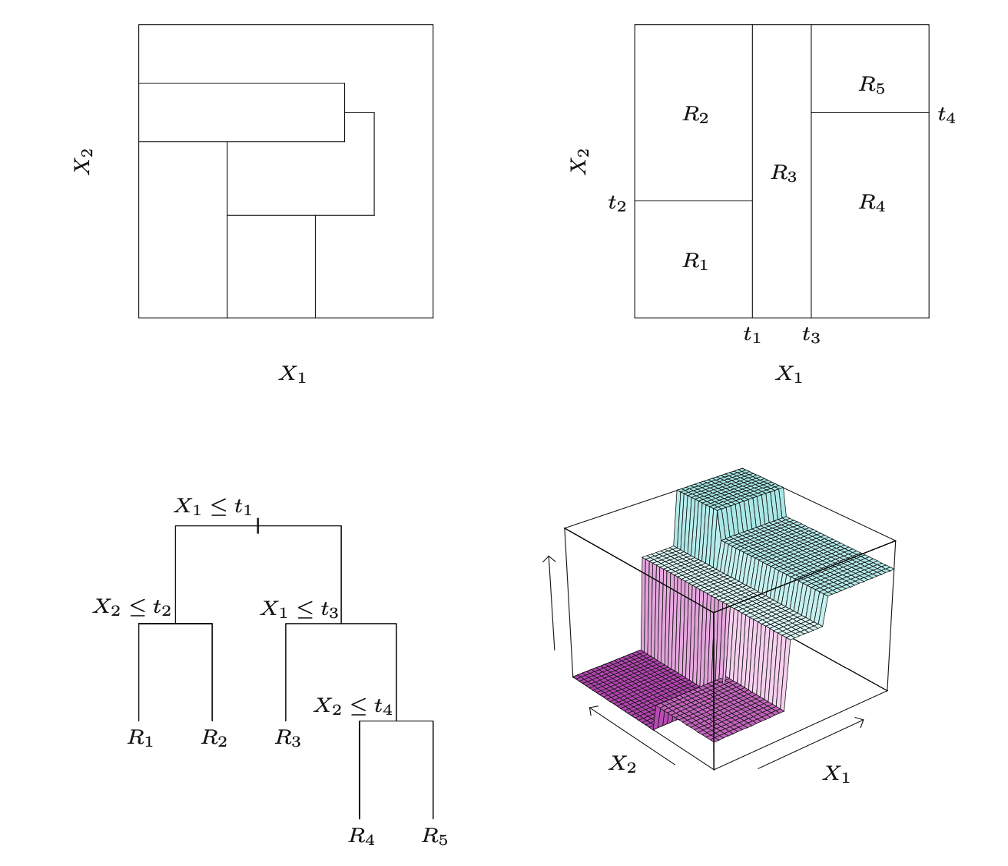
\includegraphics[width=0.94\textwidth]{illuTree.png}
  \caption{A generic partition, a recursive rectangular partition, its tree
  representation, and the resulting piecewise-constant fit.  Adapted from
  Friedman, Hastie, and Tibshirani, \emph{The Elements of Statistical Learning}
  (2009), p.~306.}
  \label{fig:cf-tree}
\end{figure}

In Figure~\ref{fig:cf-tree}, the top-left partition is not generally representable
by recursive one-coordinate splits.  The top-right partition is; the bottom-left
panel records the corresponding decision rules, and the bottom-right panel shows
the fitted step function.

\subsection{From a regression tree to a causal tree}
\label{sec:cf-causal-tree}

A causal tree targets the contrast in \eqref{eq:cf-identification}, not merely an
outcome mean.  In a simple description, each proposed child node contains a treated
mean and a control mean, and hence an estimated treatment effect.  A useful split is
one for which the treatment-effect estimates differ substantially across the two
children, subject to penalties for estimation noise and constraints ensuring that
both treatment arms are represented.

This description conveys the intuition, but production implementations use more
carefully regularized splitting objectives than the raw squared difference between
two noisy effect estimates.

\subsection{Honesty}
\label{sec:cf-honesty}

If the same outcomes select the partition and estimate effects inside the selected
leaves, the procedure can chase noise.  Conditional on the selected leaf, the
within-leaf outcomes are no longer an ordinary, exogenously selected sample.
\emph{Honesty} separates the two tasks:

\begin{enumerate}
  \item randomly divide a subsample into a splitting sample and an estimation
  sample;
  \item use only the splitting sample to construct the tree;
  \item hold the partition fixed and use only the estimation sample to estimate
  effects inside its leaves.
\end{enumerate}

Under suitable regularity conditions---including overlap, regular splits, growing
leaf information, and smoothness---honest tree and forest estimators can be shown
to be consistent and asymptotically normal.  These are asymptotic statements, not a
claim of exact finite-sample unbiasedness.  Pointwise nonparametric rates are
typically slower than the parametric $n^{-1/2}$ rate.

\subsection{Causal forests}

A single causal tree is unstable: a modest change in the data can alter an early
split and therefore the entire partition.  A causal forest averages many randomized
honest trees:

\begin{enumerate}
  \item draw a subsample of the observations;
  \item grow an honest causal tree, usually considering a random subset of
  covariates at each split;
  \item repeat for $B$ trees;
  \item average the $B$ tree predictions at the target $w$.
\end{enumerate}

Subsampling and random covariate selection make the trees less correlated; averaging
then stabilizes the prediction.  Across trees, an observation may be used for
splitting in some trees, effect estimation in others, and omitted from still others.

Three tuning ideas are especially important:

\begin{description}
  \item[Covariate subsampling.] Considering only a random subset of the $p$
  covariates at a split reduces computation and decorrelates the trees.  The
  \texttt{grf} package chooses sensible defaults that can be tuned.
  \item[Minimum leaf size.] Large leaves can smooth over real heterogeneity; tiny
  leaves have noisy treated and control means.
  \item[Balanced splits.] Each child needs enough observations, including enough
  treated and control observations, for stable effect estimation and overlap.
\end{description}

\subsection{Why ordinary linear regression is not enough}

Under complete randomization, the treatment coefficient in a short regression
identifies the ATE even if the outcome model is nonlinear.  CATE is different: it is
a function of $W$.  A linear interaction model such as
\[
  Y=\alpha+D\tau+W'\beta+D W'\delta+u
\]
restricts the CATE to $\tau+W'\delta$.  If the true CATE is nonlinear, this function
is misspecified.  Moreover, under unconfoundedness $D$ may be related to $W$, so
omitted nonlinear functions of $W$ can also confound treatment.  Causal forests
allow flexible nonlinearities and interactions, though they do not remove the need
for unconfoundedness and overlap.

\section{Implementation with \texttt{grf}}
\label{sec:cf-implementation}

The next simulation has $n=2{,}000$, ten covariates, and a treatment probability
that changes with $W_1$.  The outcome model is
\[
  Y=\max\{W_1,0\}D+W_2+\min\{W_3,0\}+\varepsilon,
\]
so the true CATE is $\tau(w)=\max\{w_1,0\}$.

\begin{rcode}
library(grf)
library(DiagrammeR)

set.seed(5280)
n <- 2000
p <- 10
W <- matrix(rnorm(n * p), nrow = n, ncol = p)
D <- rbinom(n, 1, 0.4 + 0.2 * (W[, 1] > 0))
Y <- pmax(W[, 1], 0) * D + W[, 2] + pmin(W[, 3], 0) + rnorm(n)

W_test <- matrix(0, nrow = 101, ncol = p)
W_test[, 1] <- seq(-2, 2, length.out = 101)

# A quick exploratory forest and one of its trees
forest_quick <- causal_forest(W, Y, D)
plot(get_tree(forest_quick, 1))

# A larger forest for final estimates and variance estimates
forest_full <- causal_forest(W, Y, D, num.trees = 4000)
pred <- predict(forest_full, W_test, estimate.variance = TRUE)
se <- sqrt(pred$variance.estimates)

plot(W_test[, 1], pred$predictions,
     ylim = range(pred$predictions - 1.96 * se,
                  pred$predictions + 1.96 * se, 0, 2),
     xlab = expression(W[1]), ylab = "CATE", type = "l")
lines(W_test[, 1], pred$predictions + 1.96 * se, lty = 2)
lines(W_test[, 1], pred$predictions - 1.96 * se, lty = 2)
lines(W_test[, 1], pmax(W_test[, 1], 0), col = 2)
legend("topleft", c("forest", "95% pointwise interval", "truth"),
       lty = c(1, 2, 1), col = c(1, 1, 2), bty = "n")
\end{rcode}

Four thousand trees reduce Monte Carlo noise in variance estimates but can be slow
in a browser.  The live companion uses fewer trees for a quick classroom
demonstration; the substantive workflow should use more trees and check that results
are stable as \texttt{num.trees} increases.

We can also revisit the survey-wording experiment from
Section~\ref{sec:rct-gss}.  Here the test grid fixes age at 30 and varies education.

\begin{rcode}
gss <- read.csv("data/welfare-small.csv")
Y <- as.numeric(gss$Y)
D <- as.numeric(gss$D)
W <- as.matrix(gss[, c("age", "educ")])

W_test <- cbind(age = 30,
                educ = seq(min(gss$educ), max(gss$educ), by = 1))

forest_gss <- causal_forest(W, Y, D, num.trees = 4000)
pred_gss <- predict(forest_gss, W_test, estimate.variance = TRUE)
se_gss <- sqrt(pred_gss$variance.estimates)

plot(W_test[, "educ"], pred_gss$predictions,
     ylim = range(pred_gss$predictions - 1.96 * se_gss,
                  pred_gss$predictions + 1.96 * se_gss),
     xlab = "Education", ylab = "Estimated CATE", type = "l")
lines(W_test[, "educ"], pred_gss$predictions + 1.96 * se_gss, lty = 2)
lines(W_test[, "educ"], pred_gss$predictions - 1.96 * se_gss, lty = 2)
\end{rcode}

The confidence limits above are pointwise.  They should not be interpreted as a
simultaneous confidence band for the whole CATE curve.  In an observational
application, predictive fit also cannot validate unconfoundedness.

\section{Summary}

\begin{itemize}
  \item The CATE organizes treatment-effect heterogeneity by pre-treatment
  characteristics, and averaging it recovers the ATE.
  \item Unconfoundedness and overlap identify the CATE as a contrast of two
  observable conditional means.
  \item Conventional nonparametric methods face the curse of dimensionality; a
  local estimator's standard error is typically of order $(nh^p)^{-1/2}$.
  \item Causal trees learn adaptive regions targeted to treatment-effect
  heterogeneity.  Honesty separates partition selection from effect estimation.
  \item Causal forests average many randomized honest trees, improving stability
  and permitting pointwise inference under regularity conditions.
  \item Flexible algorithms do not make causal assumptions disappear: credible
  unconfoundedness, overlap, SUTVA, and a clearly defined target population remain
  essential.
\end{itemize}

\chapter{Doubly Robust Learning}
\label{chap:doubly-robust}

\section*{Outline}

Chapter~\ref{chap:causal-forest} identified conditional treatment effects under
unconfoundedness.  We now return to the average treatment effect (ATE).  Ordinary
least squares need not recover the ATE when treatment is only conditionally random.
We develop outcome-regression and inverse-propensity-weighting representations, then
combine them in the augmented inverse propensity weighted (AIPW) score.  Cross-fitting
makes this score compatible with flexible machine-learning estimates of nuisance
functions.

\section{ATE under unconfoundedness and the failure of OLS}
\label{sec:dr-ols}

Let $W_i$ contain pre-treatment covariates.  We maintain consistency, i.i.d.
sampling, unconfoundedness,
\begin{equation}
  D_i\indep\bigl(Y_i(1),Y_i(0)\bigr)\mid W_i,
  \label{eq:dr-unconfoundedness}
\end{equation}
and overlap,
\begin{equation}
  0<e(W_i)<1\quad\text{almost surely},
  \qquad e(w)=\Pr(D_i=1\mid W_i=w).
  \label{eq:dr-overlap}
\end{equation}
Define the outcome regressions
\begin{equation}
  \mu_d(w)=\E[Y_i\mid D_i=d,W_i=w],\qquad d\in\{0,1\}.
  \label{eq:dr-outcome-regressions}
\end{equation}
By the CATE identification argument,
\begin{equation}
  \tau\equiv\operatorname{ATE}
  =\E[\mu_1(W_i)-\mu_0(W_i)].
  \label{eq:dr-gformula}
\end{equation}
This is often called the outcome-regression formula, the g-formula, or
standardization.

Identification does not imply that an arbitrary linear regression is correctly
specified.  Consider the following data-generating process.  Treatment depends on
$W$, so it is not completely randomized, but the independent variable $V$ makes
treatment random conditional on $W$.  The individual effect is $1+W^2$, hence the
ATE is $1+\E[W^2]=2$.

\begin{rcode}
library(lmtest)
library(sandwich)

set.seed(5280)
n <- 5000
W <- rnorm(n)
V <- rnorm(n)
D <- as.integer(W + V > 0)
epsilon <- rnorm(n)
Y <- 1 + D + W + D * W^2 + sin(W) + epsilon

fit_short <- lm(Y ~ D)
fit_linear <- lm(Y ~ D + W)
coeftest(fit_short, vcov. = vcovHC(fit_short, type = "HC2"))["D", ]
coeftest(fit_linear, vcov. = vcovHC(fit_linear, type = "HC2"))["D", ]
\end{rcode}

Both regressions omit nonlinear terms that are related to treatment.  Their treatment
coefficients are therefore not generally the ATE.  Adding a sufficiently rich and
correctly specified outcome model could solve the problem, but we would like a
method that accommodates flexible estimation and offers protection against one
nuisance model being misspecified.

\section{The propensity score and two representations of the ATE}
\label{sec:dr-identification}

The function $e(W_i)$ in \eqref{eq:dr-overlap} is the \emph{propensity score}.  It
summarizes how observed covariates predict treatment.  Under complete randomization
it is constant; under conditional randomization it may vary with $W_i$.

\subsection{The balancing-score result}

Rosenbaum and Rubin's balancing-score theorem states that
\begin{equation}
  D_i\indep\bigl(Y_i(1),Y_i(0)\bigr)\mid e(W_i)
  \label{eq:dr-ps-unconfoundedness}
\end{equation}
whenever \eqref{eq:dr-unconfoundedness} holds.  To see the key argument, let
$Z_i=(Y_i(1),Y_i(0))$.  Since $D_i$ is binary,
\begin{align*}
  \Pr(D_i=1\mid Z_i,e(W_i))
  &=\E[D_i\mid Z_i,e(W_i)]\\
  &=\E\!\left[\E[D_i\mid Z_i,W_i]\mid Z_i,e(W_i)\right]\\
  &=\E[e(W_i)\mid Z_i,e(W_i)]
   =e(W_i),
\end{align*}
where unconfoundedness gives the third line.  Likewise,
$\Pr(D_i=1\mid e(W_i))=e(W_i)$.  Thus the conditional treatment probability does
not depend on $Z_i$ once the propensity score is held fixed.

The theorem makes a high-dimensional conditioning problem scalar, but it does not
mean that one can ignore $W$ when estimating the propensity score.  Misspecifying
$e(W)$ can still invalidate a propensity-score analysis.

\subsection{Inverse propensity weighting}

The ATE also has the representation
\begin{equation}
  \tau
  =\E\!\left[
      \frac{D_iY_i}{e(W_i)}
      -\frac{(1-D_i)Y_i}{1-e(W_i)}
    \right].
  \label{eq:dr-ipw-id}
\end{equation}
For the treated component, consistency and iterated expectations give
\begin{align*}
  \E\!\left[\frac{D_iY_i}{e(W_i)}\right]
  &=\E\!\left[\frac{D_iY_i(1)}{e(W_i)}\right]\\
  &=\E\!\left[
      \frac{\E[D_iY_i(1)\mid W_i]}{e(W_i)}
    \right]\\
  &=\E\!\left[
      \frac{\E[D_i\mid W_i]\E[Y_i(1)\mid W_i]}{e(W_i)}
    \right]\\
  &=\E[Y_i(1)].
\end{align*}
The third line uses unconfoundedness.  The control component similarly equals
$\E[Y_i(0)]$, proving \eqref{eq:dr-ipw-id}.  Overlap is needed because the
denominators must be defined; near-zero denominators also explain why weak overlap
can make IPW unstable.

We now have two identification formulas: outcome regression in
\eqref{eq:dr-gformula} and IPW in \eqref{eq:dr-ipw-id}.  AIPW combines them.

\section{The AIPW score and double robustness}
\label{sec:dr-aipw}

For generic functions $m_1,m_0$, and $q$ taking values strictly between zero and
one, define
\begin{equation}
  \psi(O_i;m_1,m_0,q)
  =m_1(W_i)-m_0(W_i)
   +\frac{D_i\{Y_i-m_1(W_i)\}}{q(W_i)}
   -\frac{(1-D_i)\{Y_i-m_0(W_i)\}}{1-q(W_i)},
  \label{eq:dr-score}
\end{equation}
where $O_i=(Y_i,D_i,W_i)$.  If the true nuisance functions
$\eta_0=(\mu_1,\mu_0,e)$ were known, the oracle estimator would be
\begin{equation}
  \widehat\tau^*_{\mathrm{AIPW}}
  =\frac1n\sum_{i=1}^n\psi(O_i;\mu_1,\mu_0,e).
  \label{eq:dr-oracle-aipw}
\end{equation}

The augmentation terms have conditional mean zero.  For example,
\[
  \E\!\left[
    \frac{D_i\{Y_i-\mu_1(W_i)\}}{e(W_i)}\Bigm|W_i
  \right]=0.
\]
Hence $\E[\psi(O_i;\eta_0)]=\tau$.  The score can also be rearranged as
\begin{align}
  \psi(O_i;m_1,m_0,q)
  ={}&\frac{D_iY_i}{q(W_i)}
      -\frac{(1-D_i)Y_i}{1-q(W_i)} \notag\\
    &+m_1(W_i)\left\{1-\frac{D_i}{q(W_i)}\right\}
      -m_0(W_i)\left\{1-\frac{1-D_i}{1-q(W_i)}\right\}.
  \label{eq:dr-score-ipw-form}
\end{align}

These two forms reveal \emph{double robustness}:

\begin{itemize}
  \item If $m_d=\mu_d$ for $d=0,1$, then the residual augmentation terms in
  \eqref{eq:dr-score} have conditional mean zero for any admissible $q$.
  Therefore $\E[\psi]=\E[\mu_1(W)-\mu_0(W)]=\tau$.
  \item If $q=e$, then
  \[
    \E\!\left[1-\frac{D}{e(W)}\Bigm|W\right]=0,
    \qquad
    \E\!\left[1-\frac{1-D}{1-e(W)}\Bigm|W\right]=0.
  \]
  Consequently, the last line of \eqref{eq:dr-score-ipw-form} has mean zero for
  any integrable $m_1,m_0$, while its first line identifies the ATE.
\end{itemize}

The conditioning on $W$ in the second argument is essential: an unconditional
mean-zero equality alone would not justify multiplication by an arbitrary function
of $W$.

Let $\widehat\mu_d$ and $\widehat e$ be estimated nuisance functions.  The plug-in
AIPW estimator is
\begin{equation}
  \widehat\tau_{\mathrm{AIPW}}
  =\frac1n\sum_{i=1}^n
  \psi(O_i;\widehat\mu_1,\widehat\mu_0,\widehat e).
  \label{eq:dr-feasible-aipw}
\end{equation}
Subject to regularity conditions, it remains consistent when either both outcome
regressions are consistently estimated or the propensity score is consistently
estimated.  Double robustness protects against one class of nuisance-model
misspecification; it does not protect against violations of unconfoundedness,
overlap, consistency, or sampling assumptions.

\section{Cross-fitting and double machine learning}
\label{sec:dr-dml}

Flexible machine-learning estimates can overfit.  Evaluating a nuisance function on
the same observations used to train it creates dependence that complicates the
first-order expansion of \eqref{eq:dr-feasible-aipw}.  \emph{Cross-fitting} removes
this own-observation link.

Partition the sample into $K$ folds $I_1,\ldots,I_K$.  For each fold $k$:

\begin{enumerate}
  \item estimate $\mu_1$, $\mu_0$, and $e$ using observations outside $I_k$;
  call the resulting functions
  $\widehat\mu_1^{(-k)},\widehat\mu_0^{(-k)},\widehat e^{(-k)}$;
  \item evaluate those functions for observations $i\in I_k$ and compute their
  AIPW scores.
\end{enumerate}

The cross-fitted estimator is
\begin{equation}
  \widehat\tau_{\mathrm{DML}}
  =\frac1n\sum_{k=1}^K\sum_{i\in I_k}
  \psi\!\left(O_i;widehat\mu_1^{(-k)},
  \widehat\mu_0^{(-k)},\widehat e^{(-k)}\right).
  \label{eq:dr-dml}
\end{equation}
Every observation is used for score evaluation once and for nuisance training in
the other folds.

Why can slowly estimated nuisance functions still yield root-$n$ inference for
$\tau$?  The AIPW score is orthogonal: its population expectation is locally
insensitive, to first order, to small perturbations of the nuisance functions.  The
leading remainder is governed by a \emph{product} of nuisance errors.  A typical
sufficient condition is
\begin{equation}
  \|\widehat e-e\|_2
  \left(\|\widehat\mu_1-\mu_1\|_2+
        \|\widehat\mu_0-\mu_0\|_2\right)
  =o_p(n^{-1/2}),
  \label{eq:dr-product-rate}
\end{equation}
together with consistent nuisance estimates, bounded moments, and strong overlap:
$e(W)$ is bounded away from zero and one.

If the propensity and outcome-regression mean-squared errors are respectively of
orders $n^{-a}$ and $n^{-b}$, their $L^2$ errors have orders $n^{-a/2}$ and
$n^{-b/2}$.  Thus \eqref{eq:dr-product-rate} corresponds to $a+b>1$ when these are
exact big-$O$ rates; an equality case needs a stronger little-$o$ statement.  It is
incorrect simply to compare nuisance variances with $1/n$ without taking square
roots and the product remainder into account.

Under appropriate conditions,
\begin{equation}
  \sqrt n(\widehat\tau_{\mathrm{DML}}-\tau)
  \dto \N(0,V_{\mathrm{eff}}),
  \qquad
  V_{\mathrm{eff}}=\Var\{\psi(O_i;\eta_0)\}.
  \label{eq:dr-dml-clt}
\end{equation}
The centered score $\psi(O_i;\eta_0)-\tau$ is the efficient influence function for
the ATE in the nonparametric unconfoundedness model.  Consequently, an estimator
with the expansion in \eqref{eq:dr-dml-clt} attains the semiparametric efficiency
bound among regular estimators in that model.  This is a precise efficiency claim,
not a statement that AIPW is unconditionally ``best'' in every finite sample.

An estimated standard error is obtained from the sample variance of the cross-fitted
scores:
\begin{equation}
  \widehat{\operatorname{se}}(\widehat\tau_{\mathrm{DML}})
  =\sqrt{\frac{1}{n(n-1)}
    \sum_{i=1}^n(\widehat\psi_i-\widehat\tau_{\mathrm{DML}})^2}.
  \label{eq:dr-dml-se}
\end{equation}
The familiar Wald confidence interval then applies when the asymptotic conditions
are credible.

\section{Implementation with generalized random forests}
\label{sec:dr-implementation}

The \texttt{grf} package estimates nuisance components internally and uses
out-of-bag predictions to construct an orthogonalized ATE estimate.  We return to
the simulation from Chapter~\ref{chap:causal-forest}.

\begin{rcode}
library(grf)

set.seed(5280)
n <- 2000
p <- 10
W <- matrix(rnorm(n * p), nrow = n, ncol = p)
D <- rbinom(n, 1, 0.4 + 0.2 * (W[, 1] > 0))
Y <- pmax(W[, 1], 0) * D + W[, 2] + pmin(W[, 3], 0) + rnorm(n)

# Use many trees for stable final inference.
forest <- causal_forest(W, Y, D, num.trees = 4000)
average_treatment_effect(
  forest,
  target.sample = "all",
  method = "AIPW"
)
\end{rcode}

Here the true ATE is
$\E[\max\{W_1,0\}]=1/\sqrt{2\pi}\approx0.399$.  Comparing the estimate with this
truth is a useful simulation check.  Four thousand trees are appropriate for a
substantive analysis but unnecessarily slow for a short browser demonstration; the
live companion uses a smaller forest and labels that choice explicitly.

In applied work, also inspect the estimated propensity scores, sensitivity to
forest tuning, and the effective target population.  Extreme propensities can make
AIPW noisy despite its robustness properties.  If overlap is poor, changing the
estimand, trimming by a pre-specified rule, or collecting better comparison data may
be more defensible than relying on a few enormous weights.

\section{Summary}

\begin{itemize}
  \item Under unconfoundedness and overlap, the ATE has both an outcome-regression
  representation and an inverse-propensity-weighted representation.
  \item OLS with an arbitrary linear specification need not estimate the ATE when
  treatment depends on covariates.
  \item AIPW combines the two representations and is consistent if either the two
  outcome regressions or the propensity score is consistently estimated, subject
  to regularity conditions.
  \item Cross-fitting permits flexible nuisance learners while avoiding
  own-observation overfitting in the score.
  \item Orthogonality makes the leading bias depend on the product of nuisance
  errors.  With strong overlap and suitable product rates, AIPW is root-$n$ normal
  and semiparametrically efficient.
  \item These statistical protections do not repair a failure of the identifying
  causal assumptions.
\end{itemize}

\chapter{Sharp Regression Discontinuity Designs}
\label{chap:rd}

\begin{description}
  \item[Motivation.] What can we learn when treatment is a deterministic
  function of a running variable?
  \item[Identification.] Why only the treatment effect at the cutoff is
  identified without additional assumptions.
  \item[Estimation.] How local linear regression estimates the two limits.
  \item[Application.] Incumbency effects in U.S. House elections.
\end{description}

\section{A deterministic treatment rule}

In earlier chapters, unconfoundedness was paired with overlap.  For a scalar
covariate $W_i$, those assumptions allowed us to compare treated and untreated
units at the same value $W_i=w$.  A sharp regression discontinuity (RD) design
is deliberately different.  Treatment obeys a deterministic rule,
\begin{equation}
  D_i=\1\{W_i\geq c\},
  \label{eq:rd-assignment}
\end{equation}
where $c$ is a known cutoff.  Conditional on $W_i$, treatment is degenerate;
there is no treated--untreated overlap except in a limiting sense at the
cutoff.  Thus the usual unconfoundedness formula
\[
  \E[Y_i\mid D_i=1,W_i=w]-\E[Y_i\mid D_i=0,W_i=w]
\]
is not well-defined: below $c$ the first conditional mean is unavailable, and
above $c$ the second is unavailable.

Write the observed outcome as
\[
  Y_i=D_iY_i(1)+(1-D_i)Y_i(0).
\]
The conditional average treatment effect is
\begin{equation}
  \tau(w)=\E[Y_i(1)-Y_i(0)\mid W_i=w].
  \label{eq:rd-cate}
\end{equation}
Away from the cutoff, one of its two components is missing:
\[
  \tau(w)=
  \begin{cases}
    \E[Y_i\mid W_i=w]-\E[Y_i(0)\mid W_i=w], & w\geq c,\\
    \E[Y_i(1)\mid W_i=w]-\E[Y_i\mid W_i=w], & w<c.
  \end{cases}
\]
Without extrapolation, therefore, we cannot identify the entire function
$\tau(\cdot)$ or the population ATE.

\section{Identification at the cutoff}
\label{sec:rd-identification}

The cutoff is special because observations can approach it from either side.
Assume that
\[
  m_d(w)=\E[Y_i(d)\mid W_i=w],\qquad d\in\{0,1\},
\]
is continuous at $c$.  Equation~\eqref{eq:rd-assignment} and consistency imply
\begin{align*}
  \lim_{w\downarrow c}\E[Y_i\mid W_i=w]&=m_1(c),\\
  \lim_{w\uparrow c}\E[Y_i\mid W_i=w]&=m_0(c).
\end{align*}
Here $w\downarrow c$ approaches from above, whereas $w\uparrow c$ approaches
from below.  Subtracting the two limits identifies
\begin{equation}
  \tau_{RD}
  \equiv \E[Y_i(1)-Y_i(0)\mid W_i=c]
  =\lim_{w\downarrow c}\E[Y_i\mid W_i=w]
   -\lim_{w\uparrow c}\E[Y_i\mid W_i=w].
  \label{eq:sharp-rd-identification}
\end{equation}

\begin{important}
RD identification comes from the deterministic assignment rule and continuity
of the untreated and treated conditional means at the cutoff.  It does not
come from the usual unconfoundedness-plus-overlap argument.
\end{important}

The continuity requirement says that, absent the change in treatment status,
the expected outcome would not jump exactly at $c$.  This is plausible when
units just above and just below the threshold are otherwise comparable.  It is
not automatic.  Other programs changing at the same cutoff, precise
manipulation of $W_i$, or a discontinuous change in the composition of units
can invalidate the design.

The estimand is local.  An RD study of a program with an income threshold
$c=\$1{,}000$, for example, estimates the effect for families at that
threshold.  It does not by itself identify the effect for families earning
$\$500$.  Whether $\tau_{RD}$ is substantively interesting is therefore a
design question, not a statistical one.

\section{Local linear estimation}
\label{sec:rd-local-linear}

Equation~\eqref{eq:sharp-rd-identification} asks for two boundary values of a
conditional mean.  Near the cutoff, approximate that mean by a different line
on each side:
\begin{align}
  Y_i&=\beta_0^+ +\beta_1^+(W_i-c)+\varepsilon_i^+,
       &&W_i\geq c,\label{eq:rd-right-line}\\
  Y_i&=\beta_0^- +\beta_1^-(W_i-c)+\varepsilon_i^-,
       &&W_i<c.\label{eq:rd-left-line}
\end{align}
Then $\beta_0^+-\beta_0^-$ approximates the discontinuity.  Equivalently, fit
one interacted regression,
\begin{equation}
  Y_i=\gamma_0+\gamma_1D_i+\gamma_2(W_i-c)
      +\gamma_3D_i(W_i-c)+\varepsilon_i,
  \label{eq:rd-local-regression}
\end{equation}
using only observations near $c$.  The mapping is
\[
  \gamma_0=\beta_0^-,\quad
  \gamma_2=\beta_1^-,\quad
  \gamma_0+\gamma_1=\beta_0^+,\quad
  \gamma_2+\gamma_3=\beta_1^+,
\]
so $\gamma_1$ is the estimated jump.

Let
\[
  X_i=\bigl(1,D_i,W_i-c,D_i(W_i-c)\bigr)',
  \qquad
  K_{hi}=K\!\left(\frac{W_i-c}{h}\right).
\]
A kernel $K$ gives greater weight to observations closer to the cutoff, and
$h>0$ is the bandwidth.  Weighted least squares solves
\begin{equation}
  \frac{1}{n}\sum_{i=1}^n K_{hi}X_i(Y_i-X_i'\widehat\gamma)=0,
  \label{eq:rd-moment}
\end{equation}
and hence
\begin{equation}
  \widehat\gamma=
  \left(\frac{1}{n}\sum_i K_{hi}X_iX_i'\right)^{-1}
  \left(\frac{1}{n}\sum_i K_{hi}X_iY_i\right).
  \label{eq:rd-wls}
\end{equation}
The RD point estimate is the second element, $\widehat\gamma_1$.

As $n$ grows, the bandwidth must shrink so the linear approximation becomes
local, but not so quickly that too few observations remain.  This creates the
usual bias--variance tradeoff:
\begin{itemize}
  \item a small $h$ reduces approximation bias but increases variance;
  \item a large $h$ uses more data but risks fitting observations for which a
        straight line is a poor approximation.
\end{itemize}
At an MSE-optimal bandwidth, the leading smoothing bias need not be negligible
for inference.  Modern practice therefore uses robust bias correction and
reports sensitivity to bandwidth and polynomial-order choices.  The older IK
bandwidth of Imbens and Kalyanaraman is useful historically, but it is not the
only or necessarily preferred modern choice.

\subsection{Covariates}

Additional pre-treatment covariates are not required for the identification
argument in Section~\ref{sec:rd-identification}.  They may improve precision
and can help diagnose whether units look comparable near the cutoff.  They
should be included in a way that preserves the local RD specification; adding
post-treatment covariates can instead change or destroy the causal estimand.

\subsection{Why not a high-order global polynomial?}

It is possible to fit separate polynomials over the entire range of $W_i$.
Such fits were common in early applications, including the descriptive Lee
figure below.  High-order global polynomials can be unstable near a boundary
and can give distant observations excessive influence.  Local linear or local
quadratic methods are normally safer for primary estimation.

\section{Application: electoral incumbency}
\label{sec:rd-lee}

Lee (2008) studies whether winning a U.S. House election raises the Democratic
candidate's vote share in the next election.  Define
\begin{itemize}
  \item the running variable as the Democratic vote-share margin in election
        $t$, recentered so zero means a tie; and
  \item the outcome as the Democratic vote share in election $t+1$.
\end{itemize}
Winning election $t$ is endogenous in the full sample: stronger candidates and
districts both win more often and perform better later.  Very close elections,
however, compare districts on opposite sides of an institutional threshold.
The discontinuity at zero in Figure~\ref{fig:rd-lee} is interpreted as the
incumbency effect under the continuity assumptions above.

\begin{figure}[tbp]
  \centering
  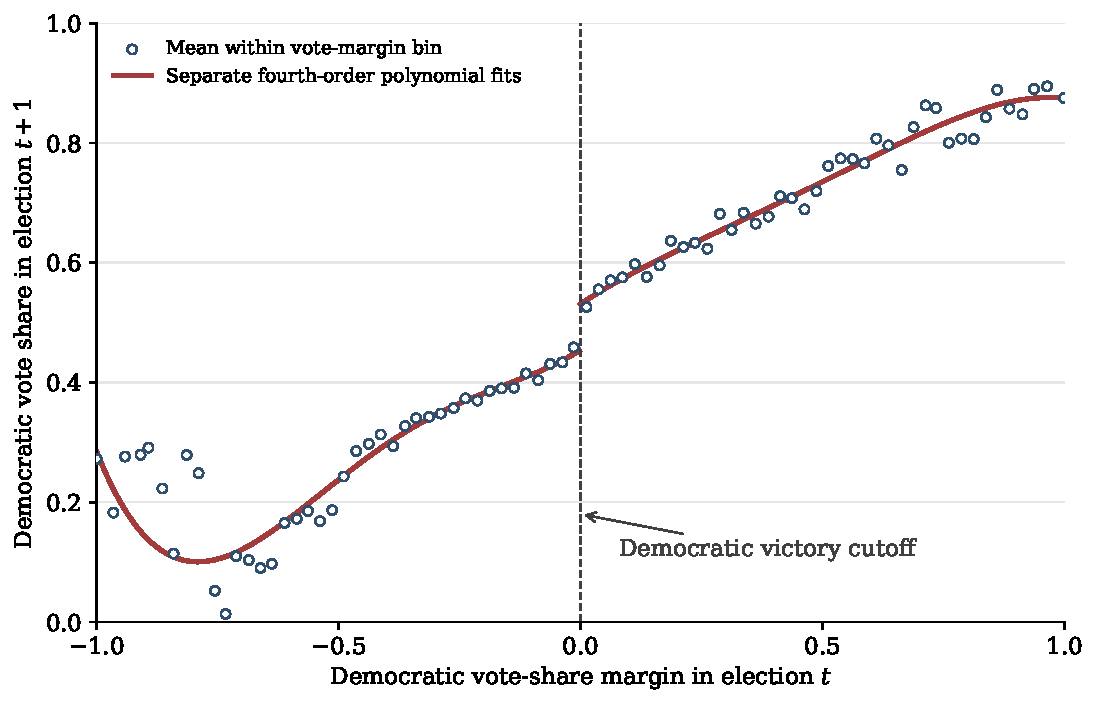
\includegraphics[width=0.88\textwidth]{../assets/Ch8RD_Lee_recreated.pdf}
  \caption{A Lee-style electoral RD illustration.  Circles are equal-width-bin
  means from the course data; curves are separate fourth-order polynomial fits
  used for visualization.  Primary estimation should use a local method.}
  \label{fig:rd-lee}
\end{figure}

Other well-known applications study mayoral wages and performance, colonial
institutions and development, financial-aid offers and college enrollment, and
angel funding and startup growth.  In every case, the central task is to defend
the institutional cutoff and the continuity of potential outcomes there.

\section{R implementation}
\label{sec:rd-r}

The following small simulation uses the \texttt{rdd} package.  Its default
\texttt{RDestimate()} call uses a triangular kernel and an automatically chosen
bandwidth.  The companion Quarto Live page runs the same code in the browser.

\begin{rcode}
library(rdd)

set.seed(5280)
x <- runif(1000, -1, 1)
y <- 3 + 2 * x + 10 * (x >= 0) + rnorm(1000)

fit_auto <- RDestimate(y ~ x)
fit_grid <- RDestimate(y ~ x,
                       bw = c(0.10, 0.20, 0.30),
                       kernel = "gaussian")
summary(fit_auto)
summary(fit_grid)
plot(fit_auto)
\end{rcode}

The Lee-style data can be loaded as follows.  The file path in the live page is
relative to the chapter file.

\begin{rcode}
library(rdd)
house <- read.csv("house.csv")
lee_local <- RDestimate(y ~ x, data = house)
summary(lee_local)
plot(lee_local)
\end{rcode}

\section*{Summary}

\begin{itemize}
  \item Sharp RD assigns treatment deterministically at a known cutoff, so
        ordinary overlap fails.
  \item Continuity identifies one local effect: the jump in the conditional
        mean of the outcome at the cutoff.
  \item Local linear regression estimates separate boundary values and avoids
        relying on a high-order global polynomial.
  \item Bandwidth choice, bias correction, manipulation, concurrent policies,
        and the local interpretation are substantive parts of the design.
\end{itemize}

\chapter{Instrumental Variables and Local Average Treatment Effects}
\label{chap:late}

\begin{description}
  \item[Motivation.] What can a randomized offer identify when people do not
  fully comply with their assignment?
  \item[LATE.] Define the causal effect for compliers and state the assumptions
  that identify it.
  \item[IV estimation.] Derive the Wald estimand and its moment-equation
  representation.
  \item[Applications.] Discuss where credible instruments come from and why
  exclusion and relevance require substantive arguments.
\end{description}

\section{Noncompliance and intent to treat}

Suppose access to an HPV vaccine is allocated by lottery.  Let $Z_i=1$ mean
that individual $i$ wins a free offer and let $D_i=1$ mean that she actually
receives the vaccine.  Even if $Z_i$ is randomized, compliance need not be
perfect:
\begin{itemize}
  \item some winners may decline the vaccine; and
  \item some nonwinners may obtain it elsewhere.
\end{itemize}
The difference
\[
  \E[Y_i\mid Z_i=1]-\E[Y_i\mid Z_i=0]
\]
is the \emph{intent-to-treat} (ITT) effect of the offer on the outcome.  It is
not generally the average effect of receiving the vaccine.

To describe noncompliance, define the potential treatment $D_i(z)$: whether
unit $i$ would receive treatment if the instrument were set to $z$.  Only one
of $D_i(0)$ and $D_i(1)$ is observed, because
\begin{equation}
  D_i=Z_iD_i(1)+(1-Z_i)D_i(0).
  \label{eq:late-observed-treatment}
\end{equation}
The pair $(D_i(0),D_i(1))$ defines four principal strata.

\begin{table}[tbp]
  \centering
  \caption{Compliance types for a binary instrument and treatment}
  \label{tab:late-types}
  \begin{tabular}{lcc}
    \toprule
    Type & $D_i(0)$ & $D_i(1)$\\
    \midrule
    Never-taker  & 0 & 0\\
    Complier     & 0 & 1\\
    Defier       & 1 & 0\\
    Always-taker & 1 & 1\\
    \bottomrule
  \end{tabular}
\end{table}

We never observe an individual's type directly.  Calling a unit a complier is
also application-specific: it depends on which direction of the instrument is
defined as encouragement.

\begin{definition}[Local average treatment effect]
For binary $Z_i$ and $D_i$, the local average treatment effect is
\begin{equation}
  LATE=\E[Y_i(1)-Y_i(0)\mid D_i(1)>D_i(0)].
  \label{eq:late-definition}
\end{equation}
It is the average treatment effect for compliers.
\end{definition}

If everyone is a complier, LATE equals the population ATE.  Otherwise it is a
local parameter for the subpopulation whose treatment status is changed by the
instrument.  Different valid instruments may therefore identify different
LATEs.

\section{Identification of LATE}
\label{sec:late-identification}

It helps to separate four assumptions that are sometimes bundled together.

\begin{enumerate}
  \item \textbf{Random assignment (instrument exogeneity):}
  \begin{equation}
    Z_i\indep\bigl(Y_i(0),Y_i(1),D_i(0),D_i(1)\bigr).
    \label{eq:late-random-assignment}
  \end{equation}
  \item \textbf{Exclusion:} the instrument affects the outcome only through
  treatment.  If outcomes were initially written $Y_i(d,z)$, exclusion says
  $Y_i(d,z)=Y_i(d)$ for every $d,z$.
  \item \textbf{Relevance:}
  \begin{equation}
    \E[D_i\mid Z_i=1]\neq \E[D_i\mid Z_i=0].
    \label{eq:late-relevance}
  \end{equation}
  \item \textbf{Monotonicity:}
  \begin{equation}
    D_i(1)\geq D_i(0)\quad\text{almost surely}.
    \label{eq:late-monotonicity}
  \end{equation}
  After orienting $Z_i$ as an encouragement, there are no defiers.
\end{enumerate}

Random assignment and exclusion are distinct.  A lottery can be randomized but
still violate exclusion if winning changes behavior through publicity, income,
or expectations even when treatment receipt is held fixed.

\begin{theorem}[Imbens--Angrist LATE theorem]
Under random assignment, exclusion, relevance, and monotonicity,
\begin{equation}
  LATE=
  \frac{\E[Y_i\mid Z_i=1]-\E[Y_i\mid Z_i=0]}
       {\E[D_i\mid Z_i=1]-\E[D_i\mid Z_i=0]}.
  \label{eq:late-wald-population}
\end{equation}
The numerator is the outcome ITT and the denominator is the first-stage ITT.
\end{theorem}

\begin{proof}
Consistency and exclusion give
$Y_i=D_iY_i(1)+(1-D_i)Y_i(0)$.  Using
Equation~\eqref{eq:late-observed-treatment} and random assignment,
\begin{align*}
  &\E[Y_i\mid Z_i=1]-\E[Y_i\mid Z_i=0]\\
  &\quad=\E\!\left[(D_i(1)-D_i(0))
                     (Y_i(1)-Y_i(0))\right].
\end{align*}
Under monotonicity, $D_i(1)-D_i(0)$ equals one for compliers and zero for
always- and never-takers.  Hence the last display equals
\[
  \Pr\{D_i(1)>D_i(0)\}
  \E[Y_i(1)-Y_i(0)\mid D_i(1)>D_i(0)].
\]
Similarly,
\begin{align*}
  \E[D_i\mid Z_i=1]-\E[D_i\mid Z_i=0]
  &=\E[D_i(1)-D_i(0)]\\
  &=\Pr\{D_i(1)>D_i(0)\}.
\end{align*}
Relevance makes this probability nonzero, so division yields
Equation~\eqref{eq:late-wald-population}.
\end{proof}

Monotonicity is substantive, not a mathematical convenience.  It can be
credible for a one-sided encouragement but implausible if the instrument pushes
different people in opposite directions.  Without monotonicity, the Wald ratio
mixes complier and defier effects with opposite signs.

\subsection{A linear moment representation}
\label{sec:late-linear}

For binary $Z_i$, define
\begin{align*}
  \gamma&=\E[D_i\mid Z_i=1]-\E[D_i\mid Z_i=0],\\
  \delta&=\E[Y_i\mid Z_i=1]-\E[Y_i\mid Z_i=0].
\end{align*}
The linear projections on $(1,Z_i)$ can be written
\begin{align*}
  D_i&=\gamma_0+\gamma Z_i+\nu_i,
       &\E[\nu_i]=\E[Z_i\nu_i]=0,\\
  Y_i&=\delta_0+\delta Z_i+\mu_i,
       &\E[\mu_i]=\E[Z_i\mu_i]=0.
\end{align*}
Because relevance implies $\gamma\neq0$, substituting the first equation into
the second produces
\begin{equation}
  Y_i=\beta_0+\beta_1D_i+\varepsilon_i,
  \qquad
  \E[\varepsilon_i]=\E[Z_i\varepsilon_i]=0,
  \label{eq:late-iv-linear}
\end{equation}
where $\beta_1=\delta/\gamma=LATE$.  In general
$\Cov(D_i,\varepsilon_i)\neq0$, which is precisely why OLS is not appropriate.

Equation~\eqref{eq:late-iv-linear} is a useful moment representation.  It does
not require the individual treatment effect to be constant or the conditional
mean of $Y_i$ to be globally linear in $D_i$.

\subsection{Conditional LATE}

Let $W_i$ contain pre-instrument covariates.  A conditional design assumes, for
example,
\[
  Z_i\indep\bigl(Y_i(0),Y_i(1),D_i(0),D_i(1)\bigr)\mid W_i,
\]
together with conditional exclusion, relevance, and monotonicity.  One possible
structural shorthand is $Y_i=g(D_i,W_i,U_i)$ and
$D_i=h(Z_i,W_i,V_i)$ with $Z_i\indep(U_i,V_i)\mid W_i$; importantly, the
treatment equation depends on $Z_i$, not on $D_i$ itself.

At covariate values with a nonzero conditional first stage,
\begin{equation}
  CLATE(w)=
  \frac{\E[Y_i\mid Z_i=1,W_i=w]-\E[Y_i\mid Z_i=0,W_i=w]}
       {\E[D_i\mid Z_i=1,W_i=w]-\E[D_i\mid Z_i=0,W_i=w]}.
  \label{eq:clate}
\end{equation}
Unlike the scalar unconditional LATE, $CLATE(w)$ is a function.  Flexible
methods such as \texttt{grf::instrumental\_forest()} can estimate heterogeneous
conditional effects under suitable conditions.

\section{Instrumental-variable estimation}
\label{sec:late-estimation}

The two moment equations associated with
Equation~\eqref{eq:late-iv-linear} are
\begin{align}
  \E[Y_i-\beta_0-\beta_1D_i]&=0,\label{eq:iv-moment-one}\\
  \E[Z_i(Y_i-\beta_0-\beta_1D_i)]&=0.\label{eq:iv-moment-two}
\end{align}
Eliminating the intercept gives
\begin{equation}
  \beta_1=\frac{\Cov(Y_i,Z_i)}{\Cov(D_i,Z_i)}.
  \label{eq:iv-covariance-ratio}
\end{equation}
For $p=\Pr(Z_i=1)$,
\begin{align*}
  \Cov(D_i,Z_i)
  &=p(1-p)\{\E[D_i\mid Z_i=1]-\E[D_i\mid Z_i=0]\},
\end{align*}
so the denominator is nonzero exactly when $0<p<1$ and the instrument is
relevant.  Replacing moments by sample averages yields
\begin{equation}
  \widehat\beta_{IV}=
  \frac{\sum_{i=1}^n(Y_i-\bar Y)(Z_i-\bar Z)}
       {\sum_{i=1}^n(D_i-\bar D)(Z_i-\bar Z)}.
  \label{eq:iv-sample-wald}
\end{equation}
With one binary instrument and one endogenous binary treatment, this is the
sample analog of the Wald ratio in
Equation~\eqref{eq:late-wald-population}.

\subsection{Weak instruments}

When the first-stage difference is close to zero, the ratio in
Equation~\eqref{eq:iv-sample-wald} is unstable.  Weak instruments can produce
substantial finite-sample bias and a poor normal approximation.  The familiar
``first-stage $F>10$'' rule is only a rough historical diagnostic, not a general
guarantee.  It depends on the number of instruments, the estimand, and the
desired tolerance for bias or size distortion.  Empirical work should report
the first stage and use weak-instrument-robust diagnostics or confidence sets
when weakness is a concern.

\section{Where do instruments come from?}
\label{sec:late-applications}

Instrumental variables transformed empirical economics, but a software command
cannot make an instrument credible.  Every application must defend both the
exclusion restriction and relevance.

\subsection{Randomized offers}

RCT assignment is an especially transparent instrument when actual treatment
has noncompliance.  For example, Kline and Walters (2016) use randomized offers
in the Head Start Impact Study to learn about early-childhood programs in the
presence of close substitutes.  The lottery identifies the effect for families
whose program participation changes because of the offer.

\subsection{Natural and quasi-experiments}

Nature or policy can generate plausibly exogenous variation.  Miguel, Satyanath,
and Sergenti (2004), for example, use rainfall shocks as an instrument for
economic growth when studying civil conflict in agriculturally dependent
African countries.  The exclusion argument is demanding: Sarsons (2015) shows
why rainfall may be related to conflict through channels other than local
income.  This exchange illustrates an important habit---actively search for
alternative pathways from $Z$ to $Y$.

Policy expansions in eligibility for maternal care provide another possible
instrument for service use.  Staggered implementation may create relevance,
but selective migration, concurrent programs, or direct income effects can
threaten exclusion.

\subsection{Variables excluded from the outcome equation}

When no experiment is available, researchers sometimes use a variable believed
to shift treatment but not the outcome directly.  Classic returns-to-schooling
examples include quarter of birth (Angrist and Krueger, 1991) and proximity to
college (Card, 1995).  Both require contestable institutional arguments:
season of birth and place of residence may be related to family background,
and their first-stage effects may be weak.

Other common constructions include reference-group variables and
``Hausman-type'' instruments, such as prices of the same product in other
markets.  Aggregation or geographic distance does not automatically guarantee
exogeneity; correlated demand shocks can invalidate the instrument.

\section{R implementation}
\label{sec:late-r}

The \texttt{ivreg} package uses the formula
\texttt{outcome \textasciitilde{} treatment \textbar{} instrument}.  The
following simulation contains never-takers, compliers, and always-takers but no
defiers.  The treatment effect is heterogeneous, so OLS and IV need not target
the same parameter.

\begin{rcode}
library(ivreg)

set.seed(5280)
n <- 4000
Z <- rbinom(n, 1, 0.5)
type <- sample(c("never", "complier", "always"), n,
               replace = TRUE, prob = c(0.25, 0.55, 0.20))

D0 <- as.integer(type == "always")
D1 <- as.integer(type %in% c("complier", "always"))
D <- ifelse(Z == 1, D1, D0)

U <- rnorm(n)
tau <- 1 + 0.7 * (type == "complier") + 0.4 * U
Y0 <- 0.5 + U + rnorm(n)
Y <- Y0 + D * tau

outcome_itt <- mean(Y[Z == 1]) - mean(Y[Z == 0])
first_stage <- mean(D[Z == 1]) - mean(D[Z == 0])
wald <- outcome_itt / first_stage
true_late <- mean(tau[type == "complier"])

c(outcome_itt = outcome_itt,
  first_stage = first_stage,
  wald = wald,
  true_late = true_late)

fit_iv <- ivreg(Y ~ D | Z)
summary(fit_iv, diagnostics = TRUE)
summary(lm(Y ~ D))
\end{rcode}

The companion Quarto Live page runs this example entirely in the browser.  In
real applications, diagnostics supplement rather than replace the design-based
arguments for random assignment, exclusion, monotonicity, and relevance.

\section*{Summary}

\begin{itemize}
  \item Random assignment identifies the ITT effect of an offer even when
        treatment receipt is endogenous.
  \item With exclusion, relevance, and monotonicity, the outcome ITT divided by
        the first-stage ITT identifies LATE for compliers.
  \item IV is a ratio estimator based on the moment condition
        $\E[Z_i\varepsilon_i]=0$; OLS fails when
        $\Cov(D_i,\varepsilon_i)\neq0$.
  \item Weak first stages make conventional normal approximations unreliable.
  \item A credible instrument requires an institutional argument, not merely a
        significant first stage.
\end{itemize}

\chapter{Neural Networks}
\label{chap:nn}

\begin{description}
  \item[Motivation.] Obtain a glimpse of how deep learning can enter modern
  econometrics.
  \item[Neural networks.] Build a flexible global approximation from simple
  layers.
  \item[Conditional expectations.] Connect squared-error training to nuisance
  functions used in causal inference.
  \item[Application.] Introduce DeepIV and large-scale heterogeneous position
  effects in sponsored search.
\end{description}

\section{Neural networks as function approximators}

Neural networks are the basic building blocks of deep learning.  They are used
for many tasks, but our focus is function approximation.  CATE and CLATE are
functions of covariates, while ATE, ATT, and LATE estimators often depend on
conditional means or probabilities.  Earlier chapters used regression trees
and forests to estimate such functions.  Neural networks provide a global,
smooth alternative.

Consider $x=(x_1,x_2,x_3)'$ and an unknown real-valued function $h(x)$.  A
one-hidden-layer network constructs a parameterized approximation
$h_\theta(x)$, as illustrated in Figure~\ref{fig:nn-schematic}.

\begin{figure}[tbp]
  \centering
  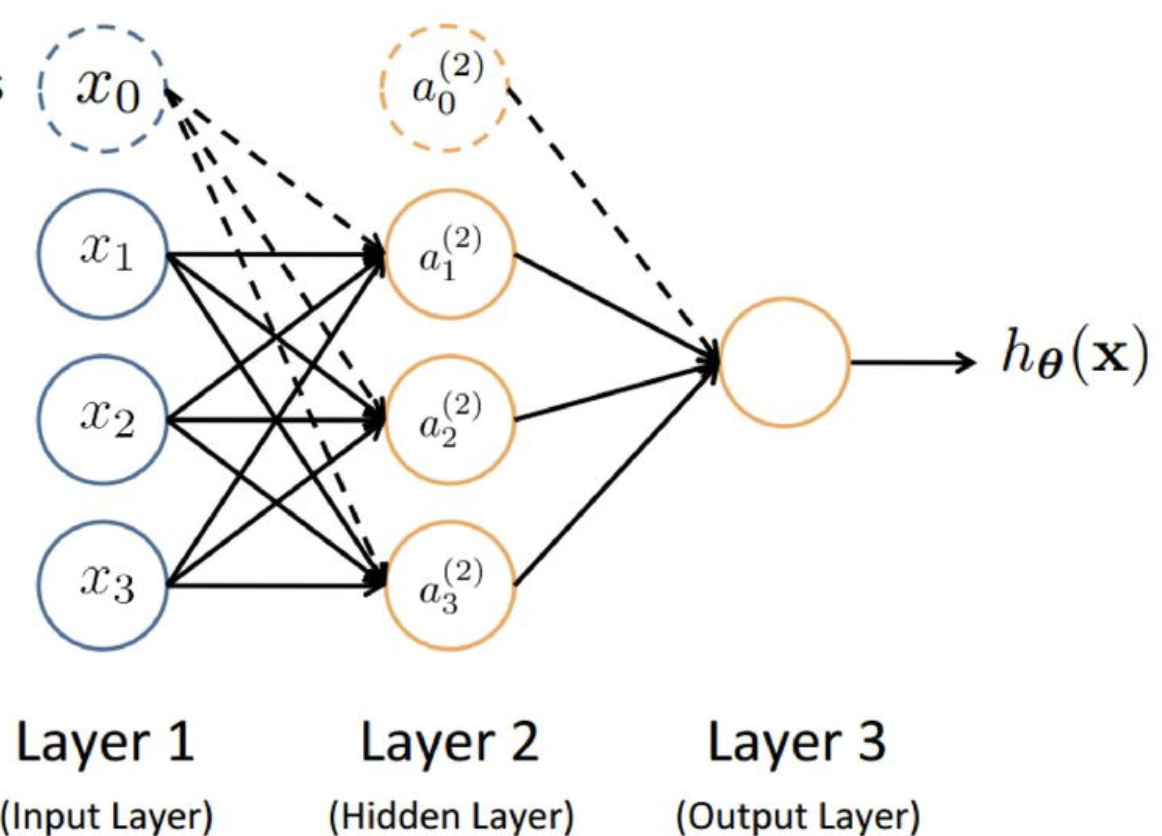
\includegraphics[width=0.78\textwidth]{../assets/NeuralNets.png}
  \caption{A one-hidden-layer feedforward neural network.  The supplied course
  illustration is based on Andrew Ng's teaching materials.}
  \label{fig:nn-schematic}
\end{figure}

Each circle is a \emph{unit} or \emph{neuron}.  Add a constant input $x_0=1$.
For hidden unit $j\in\{1,2,3\}$, define
\begin{equation}
  a_j^{(2)}=
  f^{(1)}\!\left(\theta_{0j}^{(1)}+
             \sum_{k=1}^3\theta_{kj}^{(1)}x_k\right),
  \label{eq:nn-hidden-unit}
\end{equation}
where the weighted sum is the input to the unit and $f^{(1)}$ is its activation
function.  The output is
\begin{equation}
  h_\theta(x)=
  f^{(2)}\!\left(\theta_0^{(2)}+
             \sum_{j=1}^3\theta_j^{(2)}a_j^{(2)}\right).
  \label{eq:nn-output}
\end{equation}
The network in Figure~\ref{fig:nn-schematic} has
$(3+1)\times3+(3+1)\times1=16$ weights and intercepts.

A familiar activation is the logistic, or sigmoid, function
\begin{equation}
  \sigma(z)=\frac{1}{1+e^{-z}}.
  \label{eq:nn-sigmoid}
\end{equation}
Other common choices include the rectified linear unit
$\max\{0,z\}$ and hyperbolic tangent.  For a continuous outcome, the output
activation is often the identity; for a binary probability, a sigmoid output
is natural.

\begin{example}[Approximating a binary maximum]
Let $x_1,x_2\in\{0,1\}$ and $h(x)=\max\{x_1,x_2\}$.  The single sigmoid unit
\[
  h_\theta(x)=\sigma(-20+40x_1+40x_2)
\]
is already an excellent approximation:
\begin{align*}
  h_\theta(0,0)&=\sigma(-20)\approx0,\\
  h_\theta(1,0)=h_\theta(0,1)&=\sigma(20)\approx1,\\
  h_\theta(1,1)&=\sigma(60)\approx1.
\end{align*}
The original notes used inconsistent coefficient subscripts; the expression
above uses the intercept and the two input coefficients explicitly.
\end{example}

Networks can be generalized in several directions:
\begin{itemize}
  \item a hidden layer can contain many more units than the input dimension;
  \item several hidden layers can be stacked to form a deep network;
  \item the output can be a vector, as in multiclass prediction; and
  \item inputs can include images or text after they are numerically encoded.
\end{itemize}
Universal-approximation results show that, under suitable activation and
regularity conditions, a one-hidden-layer network with sufficiently many units
can approximate a continuous function on a compact set arbitrarily well.  This
is an approximation result, not a promise that finite data and an optimization
algorithm will automatically find the best network.

For a visual experiment with architecture, activation functions, and training,
see \url{https://playground.tensorflow.org}.

\section{Conditional expectations as best predictors}
\label{sec:nn-best-predictor}

The key link with econometrics is a projection identity.  Suppose
$\E[Y^2]<\infty$.  Among all square-integrable measurable functions of $W$,
the conditional expectation minimizes mean squared error:
\begin{equation}
  m(W)=\E[Y\mid W]
  \in\arg\min_f\E[(Y-f(W))^2].
  \label{eq:nn-projection}
\end{equation}

\begin{proof}
Add and subtract $m(W)$ and expand:
\begin{align*}
  \E[(Y-f(W))^2]
  ={}&\E[(Y-m(W))^2]+\E[(m(W)-f(W))^2]\\
     &+2\E[(Y-m(W))(m(W)-f(W))].
\end{align*}
The cross term is zero because iterated expectations give
\begin{align*}
  &\E[(Y-m(W))(m(W)-f(W))]\\
  &\quad=\E\!\left[(m(W)-f(W))
        \E[Y-m(W)\mid W]\right]=0.
\end{align*}
The first term does not depend on $f$, and the second is nonnegative.  It is
minimized by $f(W)=m(W)$ almost surely.
\end{proof}

For treatment status $D\in\{0,1\}$, define
\begin{equation}
  m_d(w)=\E[Y\mid D=d,W=w].
  \label{eq:nn-treatment-regression}
\end{equation}
The corresponding population optimization problem is
\begin{equation}
  m_d(\cdot)\in
  \arg\min_h\E[(Y-h(W))^2\mid D=d].
  \label{eq:nn-population-loss}
\end{equation}
The argument of the minimum is a \emph{function}; it is not the numerical
conditional mean evaluated at one unspecified $W$.

\section{From population loss to a trained network}

Approximate $m_d(w)$ by $h_{d;\theta}(w)$.  In the subsample with $D_i=d$,
empirical risk minimization chooses
\begin{equation}
  \widehat\theta_d\in
  \arg\min_\theta
  \frac{1}{n_d}\sum_{i:D_i=d}
  \bigl(Y_i-h_{d;\theta}(W_i)\bigr)^2,
  \qquad n_d=\sum_i\1\{D_i=d\},
  \label{eq:nn-erm}
\end{equation}
and the estimated conditional mean is
$\widehat m_d(w)=h_{d;\widehat\theta_d}(w)$.  A propensity score can be trained
similarly with a binary cross-entropy loss and sigmoid output.

In practice, the numerical optimizer updates weights by backpropagation and a
gradient-based method.  Architecture, regularization, learning rate, number of
epochs, and early stopping are tuning choices.  Predictive performance should
be assessed on validation data rather than on the same observations used to
fit a highly flexible model.

\subsection{Advantages}

\begin{itemize}
  \item Networks can model nonlinearities and interactions in high-dimensional
        $W$ without specifying each one by hand.
  \item Categorical, text, and image inputs can be handled after appropriate
        numerical encoding.
  \item Matrix operations can be accelerated substantially on GPUs for large
        problems.
\end{itemize}

\subsection{Limitations and inference}

\begin{itemize}
  \item Training is nonconvex and can be sensitive to scaling, architecture,
        initialization, and regularization.
  \item A highly accurate predictor need not extrapolate well or identify a
        causal parameter when the research design is invalid.
  \item Standard errors for every point of a flexible fitted CATE surface are
        not obtained by treating network weights like coefficients in a small
        linear regression.
\end{itemize}

Neural networks can nevertheless serve as nuisance estimators inside
cross-fitted doubly robust or double-machine-learning procedures.  If the
nuisance estimates satisfy suitable rate and regularity conditions, the final
low-dimensional ATE estimator can have valid asymptotic inference even though
the individual network weights have no simple inferential interpretation.

\section{Application: DeepIV}
\label{sec:nn-deepiv}

Hartford, Lewis, Leyton-Brown, and Taddy (2017) study sponsored-search position
effects.  An advertiser's position on a Bing search page is endogenous: latent
user intent affects both placement and the probability of a click.  Their
DeepIV approach uses flexible neural networks in a nonparametric instrumental-
variables procedure.

The instruments include indicators for randomized experiments in which
advertiser--query pairs were assigned to different scoring algorithms.  These
experiments generate variation in advertisement position.  Covariates include
high-dimensional information such as the search query, and the sample exceeds
20 million observations.  The empirical analysis finds, among other results,
that a favorable position is especially valuable to small websites for
on-brand queries.

The original implementation is available at
\url{https://github.com/jhartford/DeepIV}.  It is historically important, but
software ecosystems evolve; contemporary replication should pin package
versions and test the environment before class.

\section{A small R illustration}
\label{sec:nn-r}

The following code uses the lightweight \texttt{nnet} package to approximate a
nonlinear conditional mean.  It is deliberately small enough to run through
Quarto Live in a browser.

\begin{rcode}
library(nnet)

set.seed(5280)
n <- 700
W1 <- runif(n, -1, 1)
W2 <- runif(n, -1, 1)
m <- sin(pi * W1) + W2^2
Y <- m + rnorm(n, sd = 0.25)

train <- sample(seq_len(n), 500)
dat <- data.frame(Y, W1, W2)

fit_nn <- nnet(Y ~ W1 + W2, data = dat[train, ],
               size = 8, linout = TRUE,
               decay = 0.01, maxit = 500, trace = FALSE)
fit_lm <- lm(Y ~ W1 + W2, data = dat[train, ])

test <- setdiff(seq_len(n), train)
pred_nn <- predict(fit_nn, dat[test, ])
pred_lm <- predict(fit_lm, dat[test, ])

c(neural_net = mean((Y[test] - pred_nn)^2),
  linear_model = mean((Y[test] - pred_lm)^2))
\end{rcode}

This comparison is about prediction, not causal identification.  It shows only
that a nonlinear architecture can approximate a nonlinear regression function
more flexibly than a misspecified additive linear model.

\section*{Summary}

\begin{itemize}
  \item A neural network composes weighted sums and activation functions to
        form a flexible global approximation.
  \item The conditional expectation is the population squared-error minimizer,
        which connects prediction to causal nuisance functions.
  \item Training replaces the population loss by an empirical loss and requires
        tuning, regularization, and honest validation.
  \item Neural networks do not create causal identification, but they can be
        useful nuisance estimators inside valid causal designs and cross-fitted
        doubly robust procedures.
\end{itemize}

\chapter{Difference-in-Differences and Event Studies}
\label{ch:did-event-study}
\label{chap:did}

\begin{description}
  \item[Motivation.] Policies are often adopted at different times in different
  places.  Can these timing differences reveal causal effects?
  \item[Canonical DID.] Identify an ATT with two groups, two periods, and
  parallel trends.
  \item[Staggered adoption.] Define group--time effects when cohorts adopt in
  different periods.
  \item[Modern event studies.] Avoid already-treated controls, estimate
  transparent effects first, and aggregate second.
  \item[Credibility and inference.] Understand what pre-trends, confidence
  bands, and clustered standard errors can and cannot establish.
\end{description}

\section{Motivation}

Many important treatments in economics are policies rather than randomized
experiments.  A housing subsidy, minimum-wage increase, or new technology may
be introduced in one place before another.  A simple comparison between places
with and without the policy is unlikely to be causal: adopters may have had
different outcome levels before adoption.  A before--after comparison within
adopters is also insufficient: inflation, interest rates, or a common boom may
have changed outcomes even without the policy.

Difference-in-differences (DID) combines both comparisons:
\begin{enumerate}
  \item calculate the change over time for the treated group;
  \item calculate the change for an untreated comparison group; and
  \item subtract the second change from the first.
\end{enumerate}
Permanent level differences disappear in the first difference.  Common time
changes disappear in the second.  The remaining difference is causal under a
parallel-trends assumption.

\begin{example}[A two-by-two DID]
Suppose average monthly rent is
\begin{center}
\begin{tabular}{lrrr}
  \toprule
  Group & Before & After & Change\\
  \midrule
  Cities adopting a subsidy & 120 & 134 & 14\\
  Comparison cities         & 100 & 106 &  6\\
  \bottomrule
\end{tabular}
\end{center}
The DID is
\[
  (134-120)-(106-100)=14-6=8.
\]
Under parallel trends, 6 estimates how much rent would have risen in the
adopting cities without the subsidy.  The remaining 8 is the estimated effect
on those cities.
\end{example}

\section{Two groups and two periods}
\label{sec:did-two-by-two}

Let $t\in\{0,1\}$ and define
\begin{itemize}
  \item $G_i=1$ if unit $i$ belongs to the group treated beginning in period 1;
  \item $G_i=0$ if it belongs to the never-treated control group; and
  \item $D_{it}=G_i\1\{t=1\}$ as realized treatment status.
\end{itemize}
Let $Y_{it}(1)$ denote the potential outcome under the regime ``treated
beginning in period 1'' and let $Y_{it}(0)$ denote the outcome under ``never
treated.''  The observed regime is selected by group:
\begin{equation}
  Y_{it}=G_iY_{it}(1)+(1-G_i)Y_{it}(0).
  \label{eq:did-observed-simple}
\end{equation}
The target is the post-treatment average effect on the treated,
\begin{equation}
  ATT=\E[Y_{i1}(1)-Y_{i1}(0)\mid G_i=1].
  \label{eq:did-att-simple}
\end{equation}
DID most directly learns about the group that actually adopts.  The effect for
a never-adopting group may differ and is not identified by the same comparison.

\subsection{No anticipation}

Before the policy begins, the future treatment regime should not yet affect the
outcome:
\begin{equation}
  Y_{i0}(1)=Y_{i0}(0).
  \label{eq:did-no-anticipation-simple}
\end{equation}
This can fail if firms hire in advance of an announced subsidy or households
move before a program formally starts.  The last nominally pre-treatment period
may then already be treated in an economic sense.

\subsection{Parallel trends}

The key identifying assumption is
\begin{equation}
  \E[Y_{i1}(0)-Y_{i0}(0)\mid G_i=1]
  =\E[Y_{i1}(0)-Y_{i0}(0)\mid G_i=0].
  \label{eq:did-parallel-simple}
\end{equation}
This assumption concerns \emph{changes}, not levels.  Treated and control
groups may have different average outcomes before treatment, and selection on
permanent group differences is allowed.  The assumption concerns the untreated
potential outcome; after treatment, the treated group's counterfactual path is
unobserved and cannot be checked directly.

\subsection{Identification}

Under no anticipation and parallel trends,
\begin{align}
  ATT
  &=\E[Y_{i1}-Y_{i0}\mid G_i=1]
    -\E[Y_{i1}(0)-Y_{i0}(0)\mid G_i=1]\notag\\
  &=\E[Y_{i1}-Y_{i0}\mid G_i=1]
    -\E[Y_{i1}-Y_{i0}\mid G_i=0].
  \label{eq:did-identification-simple}
\end{align}
Every term in the final line is observed.  The sample estimator is
\begin{equation}
  \widehat{ATT}_{DID}
  =(\bar Y_{11}-\bar Y_{10})-(\bar Y_{01}-\bar Y_{00}),
  \label{eq:did-estimator-simple}
\end{equation}
where $\bar Y_{gt}$ is the sample mean for group $g$ in period $t$.  The order
of differencing is immaterial:
\[
  (\bar Y_{11}-\bar Y_{10})-(\bar Y_{01}-\bar Y_{00})
  =(\bar Y_{11}-\bar Y_{01})-(\bar Y_{10}-\bar Y_{00}).
\]

\subsection{Regression representation}

With two groups and two periods, Equation~\eqref{eq:did-estimator-simple} is the
OLS coefficient $\widehat\tau$ in
\begin{equation}
  Y_{it}=\beta_0+\beta_1G_i+\beta_2Post_t
         +\tau(G_i\times Post_t)+\varepsilon_{it},
  \label{eq:did-interaction-regression}
\end{equation}
where $Post_t=\1\{t=1\}$.  With panel data, the same coefficient comes from
\begin{equation}
  Y_{it}=\alpha_i+\lambda_t+\tau D_{it}+\varepsilon_{it},
  \label{eq:did-twfe-simple}
\end{equation}
where $\alpha_i$ and $\lambda_t$ are unit and time fixed effects.  In this
canonical setting, two-way fixed effects (TWFE) is simply another way to
calculate DID.

The same units are followed over time in panel data, whereas repeated cross
sections sample different units in each period.  Both can identify ATT under
appropriate sampling and parallel-trends assumptions.  Panel data are often
more efficient because differencing removes permanent unit-specific noise.

\section{Staggered treatment adoption}
\label{sec:did-staggered}

Now let $t=1,\ldots,T$.  Define $G_i=g$ if unit $i$ is first treated in period
$g$, and $G_i=\infty$ if it is never treated.  In R code, never-treated units
are usually recorded as $G_i=0$.  With absorbing treatment,
\begin{equation}
  D_{it}=\1\{t\geq G_i\}\quad\text{for eventually treated units},
  \qquad D_{it}=0\quad\text{if }G_i=\infty.
  \label{eq:did-staggered-status}
\end{equation}
Thus $D_{it}=1$ implies $D_{i,t+1}=1$.  A treatment that repeatedly switches
on and off requires a different design or additional assumptions.

Let $Y_{it}(g)$ be the outcome if unit $i$ is first treated in period $g$, and
let $Y_{it}(0)$ be the never-treated outcome.  No anticipation requires
\begin{equation}
  Y_{it}(g)=Y_{it}(0),\qquad t<g.
  \label{eq:did-no-anticipation-staggered}
\end{equation}
The natural causal building block is the group--time effect
\begin{equation}
  ATT(g,t)=\E[Y_{it}(g)-Y_{it}(0)\mid G_i=g],
  \qquad t\geq g.
  \label{eq:did-att-gt}
\end{equation}
$ATT(4,4)$ is the adoption-period effect for cohort 4; $ATT(4,6)$ is the effect
two periods later for the same cohort; and $ATT(6,6)$ concerns another cohort
in the same calendar period.  Policy effects can vary across all these cells.

\subsection{Valid control groups}

For $ATT(g,t)$, controls must be untreated in both the baseline $g-1$ and the
comparison period $t$.  Two choices are common:
\begin{description}
  \item[Never-treated controls.] Compare cohort $g$ with units that never adopt.
  \item[Not-yet-treated controls.] Compare cohort $g$ with units treated after
  $t$, together with never-treated units.
\end{description}
The second choice uses more observations but assumes later adopters provide a
valid counterfactual trend for earlier adopters.  This is an identification
choice, not merely a software option.

With never-treated controls, assume
\begin{equation}
  \E[Y_{it}(0)-Y_{i,g-1}(0)\mid G_i=g]
  =\E[Y_{it}(0)-Y_{i,g-1}(0)\mid G_i=\infty].
  \label{eq:did-pt-never}
\end{equation}
Then
\begin{equation}
  ATT(g,t)=
  \E[Y_{it}-Y_{i,g-1}\mid G_i=g]
  -\E[Y_{it}-Y_{i,g-1}\mid G_i=\infty].
  \label{eq:did-id-never}
\end{equation}
For not-yet-treated controls, replace $G_i=\infty$ by $G_i>t$ in both displays,
using the convention that $\infty>t$.  Each $ATT(g,t)$ is then a clean
two-group, two-period DID.  Already-treated observations are not used as
untreated controls.

\subsection{Conditional parallel trends and overlap}

Let $W_i$ contain pre-treatment covariates.  A conditional assumption for
not-yet-treated controls is
\begin{align}
  &\E[Y_{it}(0)-Y_{i,g-1}(0)\mid G_i=g,W_i]\notag\\
  &\qquad=\E[Y_{it}(0)-Y_{i,g-1}(0)\mid G_i>t,W_i].
  \label{eq:did-conditional-pt}
\end{align}
Overlap requires controls at every covariate value represented in cohort $g$:
\begin{equation}
  \Pr(G_i>t\mid W_i=w)>0
  \quad\text{for }w\in\operatorname{supp}(W_i\mid G_i=g).
  \label{eq:did-overlap}
\end{equation}
Under these conditions,
\begin{align}
 ATT(g,t)=\E\Big[&
   \E[Y_{it}-Y_{i,g-1}\mid G_i=g,W_i]
   \notag\\[-2pt]
 &-\E[Y_{it}-Y_{i,g-1}\mid G_i>t,W_i]
   \ \Bigm|\ G_i=g\Big].
 \label{eq:did-conditional-id}
\end{align}
Outcome regression estimates conditional control trends; propensity weighting
reweights controls toward cohort $g$; and a doubly robust DID combines both.
Under the relevant regularity conditions, a doubly robust estimator remains
consistent if either the outcome-trend model or the generalized propensity
model is correct.  Covariates should be measured before treatment, not caused
by it.

\section{Why conventional TWFE can fail}
\label{sec:did-twfe-failure}

With many periods, researchers often estimate
\begin{equation}
  Y_{it}=\alpha_i+\lambda_t+\beta D_{it}+u_{it}.
  \label{eq:did-static-twfe}
\end{equation}
Under staggered adoption and heterogeneous effects, $\beta$ need not be an
interpretable average treatment effect.

Imagine an early-treated group E, a late-treated group L, and a never-treated
group N.  When E is newly treated, L and N are untreated.  When L is newly
treated, E is already treated.  Conventional TWFE can use all of the following:
\begin{enumerate}
  \item newly treated versus never treated;
  \item newly treated versus not yet treated; and
  \item newly treated versus already treated.
\end{enumerate}
The third comparison subtracts a change containing E's treatment-effect
dynamics.  It is not L's untreated counterfactual trend.

The Goodman--Bacon decomposition gives nonnegative weights to component
two-by-two DID comparisons, but some components use already-treated controls.
When the TWFE coefficient is instead written in terms of cohort--time treatment
effects, implicit weights can be negative.  In extreme cases, every causal
effect can be positive while the static TWFE coefficient is negative.

\subsection{Conventional event-study regressions}

A familiar dynamic regression is
\begin{equation}
  Y_{it}=\alpha_i+\lambda_t+
  \sum_{e\neq-1}\mu_e\1\{t-G_i=e\}+u_{it},
  \label{eq:did-conventional-event-study}
\end{equation}
where $e=t-G_i$ is event time and $e=-1$ is omitted.  With staggered timing and
heterogeneous effects, $\mu_e$ can be contaminated by effects at other event
times.  Even a lead can be nonzero because of post-treatment heterogeneity
rather than a genuine pre-trend.  Adding leads and lags to TWFE does not by
itself repair the control-group problem.

Fixed effects remain useful.  TWFE equals DID in the canonical two-by-two
design; a single treated cohort with a valid never-treated group avoids
already-treated controls; and a homogeneous common-effect model can justify a
static coefficient.  The lesson is to define the causal parameter and valid
controls before running the regression.

\section{Modern DID and event studies}
\label{sec:did-modern}

\begin{important}
Estimate transparent cohort--time causal effects using untreated controls, and
only then aggregate them into the summary required by the empirical question.
\end{important}

The Callaway--Sant'Anna approach estimates the collection of $ATT(g,t)$ values
using clean comparisons.  Depending on the design and covariates, each cell can
be estimated by differences in outcome changes, outcome regression, inverse
probability weighting, or doubly robust DID.

\subsection{Aggregating group--time effects}

One overall summary is
\begin{equation}
  \theta^{overall}=\sum_g\sum_{t\geq g}
  \omega_{g,t}ATT(g,t),
  \qquad \omega_{g,t}\geq0,\quad
  \sum_{g,t}\omega_{g,t}=1.
  \label{eq:did-overall-aggregation}
\end{equation}
Other summaries average within adoption cohort or within calendar period.  They
answer different questions.  Software cannot decide which is economically
relevant.

In the \texttt{did} package, \texttt{type = "simple"} weights post-treatment
cells in proportion to cohort size, so early cohorts receive more total weight
because they contribute more cells.  \texttt{type = "group"} first averages
post-treatment effects within cohort.  \texttt{type = "dynamic"} averages
contributing cohorts at each event time, using cohort-size weights.

For event time $e=t-g$, define
\begin{equation}
  \theta(e)=\sum_{g:g+e\leq T}
  \Pr(G_i=g\mid G_i+e\leq T)ATT(g,g+e).
  \label{eq:did-dynamic-aggregation}
\end{equation}
For $e\geq0$, this is the average effect after $e$ periods of exposure among
cohorts observed at that horizon.  At long horizons only early adopters remain,
so a changing curve can reflect both genuine dynamics and changing cohort
composition.  A balanced event window holds the contributing cohorts fixed,
improving comparability at the cost of discarding data.

Other modern approaches implement a similar principle in different ways:
\begin{description}
  \item[Sun--Abraham.] Estimate cohort-by-event-time interactions and aggregate
  them without contamination from other event times.
  \item[Borusyak--Jaravel--Spiess.] Fit an untreated-outcome model using
  untreated observations, impute untreated counterfactuals for treated cells,
  and average the resulting effects.
  \item[Group--time DID.] Construct clean two-by-two comparisons for each
  $(g,t)$ and then aggregate.
\end{description}
These methods can target different parameters and maintain different outcome,
comparison-group, or covariate models.  They are not interchangeable commands.

\section{Credibility and inference}
\label{sec:did-inference}

Modern event studies often report placebo or pseudo-ATT estimates before
treatment.  Large, systematic pre-treatment differences weigh against the
proposed parallel-trends design.  Estimates near zero do not prove it:
\begin{itemize}
  \item pre-treatment estimates may be noisy and have low power;
  \item paths may be parallel before treatment but diverge afterward;
  \item choosing a specification because its pre-trend test is insignificant
        changes the statistical behavior of the final estimates; and
  \item the assumption concerns an unobserved post-treatment counterfactual.
\end{itemize}
Pre-trends are a diagnostic, not a certificate of validity.

An event study reports many coefficients.  Pointwise 95\% intervals cover each
coefficient separately, not the complete curve jointly.  For statements such
as ``all pre-treatment effects are zero,'' simultaneous confidence bands are
preferable.  Modern DID packages can obtain uniform bands by multiplier
bootstrap.

Outcomes from the same unit are dependent over time.  When treatment is assigned
at a higher level, observations may also be dependent within that assignment
cluster.  With state-level policies, cluster at the state level rather than the
individual level.  With few clusters, ordinary cluster-robust approximations
may be unreliable.  The clustering level follows treatment assignment and the
dependence structure, not the number of rows.

\subsection{A design checklist}

Before estimating a staggered DID, ask:
\begin{enumerate}
  \item What is the unit, and when is it first treated?
  \item Is treatment absorbing, or can it turn off?
  \item Could units anticipate treatment?
  \item Which observations are valid controls for each cohort and period?
  \item Is parallel trends more plausible conditionally on pre-treatment
        covariates?
  \item Is the target group--time, dynamic, calendar-time, or overall ATT?
  \item Does cohort composition change across the event window?
  \item At what level should inference be clustered?
  \item Do other policies or shocks occur at the same time?
  \item Are conclusions robust to outcome scale, sample window, control group,
        and anticipation window?
\end{enumerate}

\section{R implementation}
\label{sec:did-r}

We simulate a balanced panel in which cohorts are first treated in periods 4,
6, or 8, while some units are never treated.  Treatment effects grow with
exposure and differ across cohorts---exactly the setting in which conventional
TWFE can be hard to interpret.

\subsection{Generate the panel}

\begin{rcode}
set.seed(5280)
N <- 600
TT <- 10

units <- data.frame(
  id = 1:N,
  G = sample(c(0, 4, 6, 8), N, replace = TRUE,
             prob = c(0.30, 0.25, 0.25, 0.20)),
  alpha = rnorm(N),
  W = rnorm(N)
)

data <- merge(expand.grid(id = 1:N, t = 1:TT), units,
              by = "id", sort = TRUE)
data$D <- as.integer(data$G > 0 & data$t >= data$G)
data$event_time <- ifelse(data$G > 0, data$t - data$G, NA)

data$cohort_scale <- ifelse(data$G == 4, 1.50,
                     ifelse(data$G == 6, 1.00,
                     ifelse(data$G == 8, 0.60, 0)))
data$tau <- ifelse(data$D == 1,
                   data$cohort_scale * (1 + 0.5 * data$event_time), 0)

data$lambda <- 0.25 * data$t + 0.03 * data$t^2
data$Y0 <- data$alpha + data$lambda + 0.5 * data$W +
           rnorm(nrow(data))
data$Y <- data$Y0 + data$tau
\end{rcode}

Untreated outcomes satisfy parallel trends by construction.  The treatment
effect is positive but heterogeneous across cohorts and exposure lengths.

\subsection{Calculate one group--time DID by hand}

\begin{rcode}
simple_att_gt <- function(data, g, t) {
  stopifnot(t >= g)
  base <- g - 1

  now <- data[data$t == t, c("id", "G", "Y")]
  names(now)[names(now) == "Y"] <- "Y_now"
  before <- data[data$t == base, c("id", "Y")]
  names(before)[names(before) == "Y"] <- "Y_before"

  change <- merge(now, before, by = "id")
  change$dY <- change$Y_now - change$Y_before
  treated <- change$G == g
  controls <- change$G == 0 | change$G > t

  mean(change$dY[treated]) - mean(change$dY[controls])
}

simple_att_gt(data, g = 4, t = 6)
mean(data$tau[data$G == 4 & data$t == 6])
\end{rcode}

The two numbers should be close.  The second is available only because the DGP
is known; in real data it is the unobserved causal parameter.

\subsection{Callaway--Sant'Anna group--time effects}

\begin{rcode}
library(did)

att <- att_gt(
  yname = "Y", tname = "t", idname = "id", gname = "G",
  xformla = ~ 1, data = data, panel = TRUE,
  control_group = "notyettreated", est_method = "dr",
  base_period = "universal", clustervars = "id",
  bstrap = TRUE, cband = TRUE,
  biters = 199                 # short browser demonstration only
)

summary(att)
ggdid(att)
\end{rcode}

With \texttt{xformla = \textasciitilde{} 1}, the built-in outcome-regression,
IPW, and doubly robust implementations have the same unconditional two-by-two
DID point estimates.  Replace it by, for example,
\texttt{\textasciitilde{} W} for a conditional design.

The universal base period uses $g-1$ throughout and normalizes event time $-1$
to zero.  The varying-base default leaves post-treatment effects unchanged but
uses adjacent-period comparisons for pre-treatment pseudo-ATTs.  The multiplier
bootstrap creates simultaneous bands.  We use only 199 repetitions to keep a
live classroom run short; use at least 999, and often more, for final empirical
inference.  If treatment is assigned above the unit level, specify the relevant
assignment cluster.  For panel data, \texttt{did} permits at most two cluster
variables and requires one to be the unit identifier.

\subsection{Aggregate the effects}

\begin{rcode}
overall <- aggte(att, type = "simple")
by_group <- aggte(att, type = "group")
dynamic <- aggte(att, type = "dynamic", min_e = -3, max_e = 4)

summary(overall)
summary(by_group)
summary(dynamic)
ggdid(dynamic)

dynamic_balanced <- aggte(
  att, type = "dynamic",
  min_e = -3, max_e = 3,
  balance_e = 3
)
summary(dynamic_balanced)
ggdid(dynamic_balanced)
\end{rcode}

The \texttt{simple}, \texttt{group}, and \texttt{dynamic} outputs answer
different questions and need not be numerically equal.

\subsection{Conventional and interaction-weighted event studies}

\begin{rcode}
library(fixest)

data$ever_treated <- as.integer(data$G > 0)
data$event_twfe <- ifelse(data$G > 0, data$t - data$G, 0)

twfe_event <- feols(
  Y ~ i(event_twfe, ever_treated, ref = -1) | id + t,
  data = data, cluster = ~ id
)

# A cohort outside the observed period range is treated as never treated.
data$G_sunab <- ifelse(data$G == 0, 1000, data$G)
sa_event <- feols(
  Y ~ sunab(G_sunab, t, ref.p = -1) | id + t,
  data = data, cluster = ~ id
)

iplot(list("Conventional TWFE" = twfe_event,
           "Sun--Abraham" = sa_event),
      ref.line = -1, main = "Event-study estimates")
\end{rcode}

The \texttt{fixest::iplot()} intervals here are pointwise.  They are not the
multiplier-bootstrap simultaneous bands shown by \texttt{ggdid()}.

The companion page pins WebR 0.5.9 (R 4.5), for which the WebAssembly builds of
\texttt{did}, its \texttt{fastglm} dependency, and \texttt{fixest} are mutually
compatible.  This is a runtime compatibility pin, not an econometric choice.

\section*{Summary}

\begin{itemize}
  \item DID compares outcome changes, not outcome levels.
  \item No anticipation and parallel trends for untreated potential outcomes
        identify the canonical two-by-two ATT.
  \item Under staggered adoption, $ATT(g,t)$ is the transparent causal building
        block; never-treated or not-yet-treated units can be controls.
  \item Conventional static and dynamic TWFE can be contaminated by
        already-treated comparisons when effects are heterogeneous.
  \item Modern procedures estimate valid cohort--time comparisons first and
        aggregate them second.
  \item Pre-trends, aggregation, cohort composition, anticipation, covariates,
        and clustering are substantive design choices.
\end{itemize}

\section*{Further reading}

\begin{itemize}
  \raggedright
  \item Callaway and Sant'Anna (2021), ``Difference-in-Differences with Multiple
  Time Periods,'' \emph{Journal of Econometrics},
  \url{https://doi.org/10.1016/j.jeconom.2020.12.001}.
  \item Sun and Abraham (2021), ``Estimating Dynamic Treatment Effects in Event
  Studies with Heterogeneous Treatment Effects,'' \emph{Journal of
  Econometrics}, \url{https://doi.org/10.1016/j.jeconom.2020.09.006}.
  \item Goodman-Bacon (2021), ``Difference-in-Differences with Variation in
  Treatment Timing,'' \emph{Journal of Econometrics},
  \url{https://doi.org/10.1016/j.jeconom.2021.03.014}.
  \item Borusyak, Jaravel, and Spiess (2024), ``Revisiting Event-Study Designs:
  Robust and Efficient Estimation,'' \emph{Review of Economic Studies},
  \url{https://doi.org/10.1093/restud/rdae007}.
  \item Roth, Sant'Anna, Bilinski, and Poe (2023), ``What's Trending in
  Difference-in-Differences?,'' \emph{Journal of Econometrics},
  \url{https://doi.org/10.1016/j.jeconom.2023.03.008}.
  \item Sant'Anna and Zhao (2020), ``Doubly Robust Difference-in-Differences
  Estimators,'' \emph{Journal of Econometrics},
  \url{https://doi.org/10.1016/j.jeconom.2020.06.003}.
  \item Rambachan and Roth (2023), ``A More Credible Approach to Parallel
  Trends,'' \emph{Review of Economic Studies},
  \url{https://doi.org/10.1093/restud/rdad018}.
\end{itemize}


\appendix
\chapter{Additional Matrix Algebra}
\label{app:matrix}

This appendix collects material that is useful for reference but is not
needed before the main econometrics chapters.

\section{Addition and scalar multiplication}

Matrices can be added only when they have the same dimensions, and addition
is entry by entry.  If $A$ and $B$ are $m\times k$, then
\[
  (A+B)_{ij}=a_{ij}+b_{ij}.
\]
For a scalar $c$, scalar multiplication is also entry by entry:
$(cA)_{ij}=ca_{ij}$.  Consequently,
\[
  A+B=B+A,\qquad c(A+B)=cA+cB.
\]

\section{Several views of multiplication}

Let $A$ be $n\times k$, $B$ be $n\times p$, and $C=A'B$.  In addition to
the entry formula in Chapter~\ref{ch:matrix}, we can write
\[
  C_{ab}=A_{\cdot a}'B_{\cdot b}
  \quad\text{and}\quad
  A'B=\sum_{i=1}^{n}A_iB_i',
\]
where $A_{\cdot a}$ denotes column $a$ of $A$, while $A_i$ and $B_i$ are the
column-vector versions of row $i$.  Each term $A_iB_i'$ is $k\times p$.

The following code verifies the two representations.  It is pedagogically
useful, although in practice one should use R's optimized matrix product.

\begin{rcode}
A <- matrix(c(1, 2, 3, 4, 5, 6), nrow = 3, ncol = 2)
B <- matrix(c(2, 3, 4, 5, 6, 7), nrow = 3, ncol = 2)

# Direct product
C <- t(A) %*% B

# Entry-by-entry representation
C_entry <- matrix(0, ncol(A), ncol(B))
for (a in seq_len(ncol(A))) {
  for (b in seq_len(ncol(B))) {
    C_entry[a, b] <- sum(A[, a] * B[, b])
  }
}

# Sum of row outer products
C_outer <- matrix(0, ncol(A), ncol(B))
for (i in seq_len(nrow(A))) {
  ai <- matrix(A[i, ], ncol = 1)
  bi <- matrix(B[i, ], nrow = 1)
  C_outer <- C_outer + ai %*% bi
}

C
C_entry
C_outer
\end{rcode}

\section{Rank and inverse formulas}

Some useful rank facts are
\[
  \operatorname{rank}(AB)
  \leq \min\{\operatorname{rank}(A),\operatorname{rank}(B)\}
\]
and
\[
  \operatorname{rank}(A'A)=\operatorname{rank}(AA')
  =\operatorname{rank}(A).
\]
The second equality does \emph{not} imply that both $A'A$ and $AA'$ are
invertible when $A$ is rectangular.  If $A$ is $m\times k$ with $m>k$ and
full column rank, then $A'A$ is invertible but $AA'$ has rank $k<m$ and is
singular.  The roles reverse when $m<k$ and $A$ has full row rank.

For an invertible diagonal matrix
$D=\operatorname{diag}(d_1,\ldots,d_k)$,
\[
  D^{-1}=\operatorname{diag}(d_1^{-1},\ldots,d_k^{-1}).
\]
For
\[
  A=\begin{pmatrix}a&b\\c&d\end{pmatrix},
\]
the determinant is $ad-bc$, and, when $ad-bc\neq0$,
\[
  A^{-1}=\frac{1}{ad-bc}
  \begin{pmatrix}d&-b\\-c&a\end{pmatrix}.
\]

\section{Eigenvalues and spectral decomposition}

An eigenvalue--eigenvector pair $(\lambda,v)$ of a square matrix $A$ satisfies
$Av=\lambda v$ with $v\neq0$.  A general real square matrix need not have a
full set of real eigenvectors and need not be diagonalizable.  For example,
$\begin{psmallmatrix}1&1\\0&1\end{psmallmatrix}$ is not diagonalizable.

The clean result needed most often in econometrics applies to symmetric
matrices.

\begin{theorem}[Spectral theorem]
For every real symmetric $k\times k$ matrix $A$, there are an orthogonal
matrix $H$ and a real diagonal matrix $\Lambda$ such that
\[
  A=H\Lambda H',\qquad H'H=HH'=I_k.
\]
The diagonal entries of $\Lambda$ are the eigenvalues of $A$, and the columns
of $H$ are orthonormal eigenvectors.
\end{theorem}

The decomposition is not unique: eigenvectors can be reordered, their signs
can be changed, and within an eigenspace associated with a repeated
eigenvalue, any orthonormal basis may be used.

For a real symmetric matrix:
\begin{itemize}
  \item $A$ is p.s.d. if and only if every eigenvalue is nonnegative;
  \item $A$ is p.d. if and only if every eigenvalue is positive;
  \item $\operatorname{rank}(A)$ equals the number of nonzero eigenvalues;
  \item $A$ is invertible if and only if zero is not an eigenvalue, and then
        $A^{-1}=H\Lambda^{-1}H'$.
\end{itemize}
The rank statement is not valid for every nonsymmetric matrix.  A nilpotent
matrix such as $\begin{psmallmatrix}0&1\\0&0\end{psmallmatrix}$ has rank one
but only the eigenvalue zero.

For a rectangular matrix, the analogous tool is the singular-value
decomposition $A=U\Sigma V'$.  Its rank equals the number of nonzero singular
values.  This is why singular values, rather than ordinary eigenvalues, are
the safe general-purpose rank diagnostic.

\begin{rcode}
library(Matrix)
A <- matrix(c(2, 1, 1, 2), 2, 2)
eigen(A)
rankMatrix(A)
solve(A)

# A nonsymmetric matrix that is not diagonalizable
J <- matrix(c(1, 0, 1, 1), 2, 2)
eigen(J)
\end{rcode}

\section{Matrix derivatives}

We use the convention that the gradient of a scalar-valued function with
respect to a column vector is itself a column vector.  For conformable fixed
objects $x$, $y$, and $X$,
\[
  \nabla_\beta(x'\beta)=x,
  \qquad
  \nabla_\beta(\beta'\beta)=2\beta,
  \qquad
  \frac{\partial(X\beta)}{\partial\beta'}=X.
\]
The last object is a Jacobian, not a scalar gradient.

For the least-squares criterion
\[
  Q(\beta)=(Y-X\beta)'(Y-X\beta),
\]
expansion or the chain rule gives
\begin{align*}
  \nabla_\beta Q(\beta)
  &=-2X'(Y-X\beta)\\
  &=2X'(X\beta-Y).
\end{align*}
The minus sign is essential.  Setting the gradient to zero yields the normal
equations $X'X\beta=X'Y$, and if $X$ has full column rank,
$\widehat\beta=(X'X)^{-1}X'Y$.

\section{Further reading}

Useful extensions include determinants, traces, idempotent projection
matrices, generalized inverses, and singular-value decomposition.  A compact
reference is Petersen and Pedersen's \emph{Matrix Cookbook}.

\chapter{Additional Probability and Asymptotic Tools}
\label{app:probability}

This appendix provides a more careful probability-space description, a few
distributional examples, simulation code for the WLLN and CLT, and the delta
method.  None of it is required on a first reading of
Chapter~\ref{ch:probability}.

\section{Probability spaces, events, and random variables}

A probability space is a triple $(\mathcal S,\mathcal F,P)$:
\begin{itemize}
  \item $\mathcal S$ is the \emph{sample space} of elementary outcomes;
  \item $\mathcal F$ is a sigma-algebra of events, meaning it contains
        $\mathcal S$ and is closed under complements and countable unions;
  \item $P:\mathcal F\to[0,1]$ satisfies $P(\mathcal S)=1$ and countable
        additivity over pairwise disjoint events.
\end{itemize}
A real random variable is a measurable map
$X:\mathcal S\to\mathbb R$.  Its distribution is the probability measure
induced on the real line:
\[
  P_X(B)=P\{s\in\mathcal S:X(s)\in B\}.
\]
Thus, the sample space contains underlying outcomes, whereas the support of
$X$ contains possible numerical values.  Treating those two sets as the same
is a convenient shortcut in elementary examples, but it is not the general
definition.

For example, an outcome can record tomorrow's temperature, rainfall, and
wind.  The random variable $X$ may retain only the indicator that it rains.
Then the sample space is rich, while the support of $X$ is merely $\{0,1\}$.

\section{CDFs, densities, and continuous distributions}

Every real random variable has a right-continuous c.d.f.
$F_X(x)=P(X\leq x)$.  A variable is \emph{continuous} (atomless) if
$P(X=x)=0$ for every $x$, equivalently if its c.d.f. is continuous.  It is
\emph{absolutely continuous} if there exists an integrable density $f_X$
such that
\[
  F_X(x)=\int_{-\infty}^{x}f_X(s)\,ds.
\]
Every absolutely continuous distribution is continuous, but the converse is
false.  The Cantor distribution is the standard counterexample: it has a
continuous c.d.f. but no density with respect to ordinary length (Lebesgue
measure).

The geometric ``probability equals length'' picture is therefore not a
general definition.  If $X$ is uniform on $[0,1]$, then
$P(X\in A)$ equals the length of $A$ for suitable sets $A$.  Under a
nonuniform density, probability is instead weighted length,
$P(X\in A)=\int_Af_X(x)\,dx$; for a discrete distribution, it is a sum of
point masses.

The code below compares three normal densities.  It uses base R so that the
live page loads quickly.

\begin{rcode}
x <- seq(-7, 7, length.out = 400)
plot(x, dnorm(x, 0, 1), type = "l", lwd = 2,
     xlab = "x", ylab = "density", ylim = c(0, 0.42))
lines(x, dnorm(x, 2, 1), lty = 2, lwd = 2, col = "steelblue")
lines(x, dnorm(x, 0, 2), lty = 3, lwd = 2, col = "firebrick")
legend("topright", c("N(0,1)", "N(2,1)", "N(0,4)"),
       lty = 1:3, lwd = 2,
       col = c("black", "steelblue", "firebrick"), bty = "n")
\end{rcode}

\section{Conditional distributions with continuous variables}

When $P(X=x)=0$, elementary event conditioning cannot define
$P(Y\leq y\mid X=x)$ by a ratio of probabilities.  A regular conditional
distribution supplies a mathematically valid version.  When a joint density
exists and $f_X(x)>0$, it has the familiar formula
\[
  f_{Y\mid X}(y\mid x)=\frac{f_{X,Y}(x,y)}{f_X(x)}.
\]
One sometimes motivates this expression using limits of shrinking intervals
around $x$.  Such a limit is an intuition, not a universal definition: its
validity requires regularity conditions and it identifies the conditional
law only for almost every $x$.

Bayes' rule for densities is
\[
  f_{X\mid Y}(x\mid y)
  =\frac{f_{Y\mid X}(y\mid x)f_X(x)}{f_Y(y)},
  \qquad f_Y(y)>0.
\]
Marginalization gives
\[
  f_X(x)=\int f_{X,Y}(x,y)\,dy,
  \qquad
  F_X(x)=\int F_{X\mid Y}(x\mid y)\,dF_Y(y).
\]

\section{The bivariate normal example}

A random vector $(X,Y)'$ is jointly normal if every linear combination
$aX+bY$ is normally distributed.  For a jointly normal pair, zero covariance
is equivalent to independence.  This equivalence is special: it is false for
general distributions.

The following optional demonstration plots bivariate normal densities with
positive, negative, and zero correlation.  The live version uses
\texttt{mvtnorm} and \texttt{plotly}; the two-dimensional contour option is
usually quicker in class.

\begin{rcode}
library(mvtnorm)
x <- seq(-4, 4, length.out = 80)
y <- seq(-4, 4, length.out = 80)
mu <- c(0, 0)
Sigma <- matrix(c(1, 0.5, 0.5, 1), 2, 2)
z <- outer(x, y, Vectorize(function(a, b) {
  dmvnorm(c(a, b), mean = mu, sigma = Sigma)
}))
contour(x, y, z, xlab = "X", ylab = "Y")
\end{rcode}

\section{A compact WLLN and CLT simulation}

The original classroom simulation repeated similar commands for ten sample
sizes.  The vectorized version below does the same job more transparently.
For Bernoulli$(0.5)$ observations, the WLLN predicts concentration of
$\bar X_n$ around $0.5$, and the CLT predicts
\[
  \frac{\sqrt n(\bar X_n-0.5)}{0.5}\dto N(0,1),
\]
because the Bernoulli standard deviation is $0.5$.

\begin{rcode}
set.seed(12)
B <- 1000
n_grid <- c(10, 25, 50, 100, 250)

sim_one_n <- function(n) {
  means <- replicate(B, mean(rbinom(n, 1, 0.5)))
  data.frame(
    n = n,
    mean = means,
    standardized = sqrt(n) * (means - 0.5) / 0.5
  )
}
sim <- do.call(rbind, lapply(n_grid, sim_one_n))

# WLLN: estimated probability of falling within 0.1 of the mean
aggregate(abs(mean - 0.5) < 0.1 ~ n, sim, mean)

# CLT: compare one standardized histogram with N(0,1)
z <- subset(sim, n == max(n_grid))$standardized
hist(z, probability = TRUE, breaks = 25,
     main = paste("n =", max(n_grid)), xlab = "standardized mean")
curve(dnorm(x), add = TRUE, lwd = 2, col = "firebrick")
\end{rcode}

\section{The delta method}

The delta method transfers an asymptotic distribution through a smooth
transformation.  It is a first-order Taylor expansion with probabilistic
remainder control.

\begin{theorem}[Multivariate delta method]
Suppose $X_n\in\mathbb R^k$ satisfies
\[
  \sqrt n(X_n-\theta)\dto N(0,\Sigma),
\]
and $g:\mathbb R^k\to\mathbb R^\ell$ is continuously differentiable near
$\theta$.  Let $G(\theta)$ be the $\ell\times k$ Jacobian whose $(r,j)$ entry
is $\partial g_r(\theta)/\partial\theta_j$.  Then
\[
  \sqrt n\{g(X_n)-g(\theta)\}
  \dto N\!\left(0,G(\theta)\Sigma G(\theta)'\right).
\]
\end{theorem}

For a scalar-valued $g$, $G(\theta)$ is a row vector and the limiting variance
is $G(\theta)\Sigma G(\theta)'$.  A statement such as ``converges to
$N(0,\cdot)$'' must include the $N$; a covariance matrix alone is not a
distribution.  If the first derivative is zero, this first-order result is
degenerate and a higher-order delta method may be needed.

\begin{example}[Log transformation]
If $\sqrt n(\widehat\theta-\theta)\dto N(0,V)$ with $\theta>0$, then
$g(\theta)=\log\theta$ has derivative $1/\theta$, so
\[
  \sqrt n\{\log\widehat\theta-\log\theta\}
  \dto N\!\left(0,\frac{V}{\theta^2}\right).
\]
\end{example}


\backmatter
\chapter*{Runtime and Reproducibility}
\addcontentsline{toc}{chapter}{Runtime and Reproducibility}
The source bundle includes a Quarto Live/WebR site and a two-core GitHub
Codespaces configuration. Package declarations are kept chapter-specific to
reduce browser startup time. See the project \texttt{README.md} for build and
deployment instructions.

\end{document}
